%%%%%%%%%%%%%%%%%%%%%%%%%%%%%%%%%%%%%%%%%%%%%%%%%%%%%%%%%%%%%%%%%%%%%%%%%%%%%%%
%%                                                   FORWARD BACKWARD ASYMMETRY
%%%%%%%%%%%%%%%%%%%%%%%%%%%%%%%%%%%%%%%%%%%%%%%%%%%%%%%%%%%%%%%%%%%%%%%%%%%%%%%
%%                       the chapter about the AFB and the sin2theta extraction



%______________________________________________________________________________
%                     Messung der Asymmetrie und des schwachen Mischungswinkels
\chapter{Messung der Asymmetrie und des schwachen Mischungswinkels}
\label{afb}

\begin{quote}
    The abstact comes last
\end{quote}



%______________________________________________________________________________
%                                                      Datensätze und Selektion
\section{Datensätze und Selektion}
\label{afb:selection}

% + benutzter Datensatz
% + Selektion / Akzeptanz
% + Benutzte Gewichte

% + Kontroll-Plots der Masse / Winkelverteilung / Phi

Die Messung der Vorwärts-Rückwärts Asymmetrie und die anschließende Extraktion
des schwachen Mischungswinkels basiert, wie schon die vorangegangene
Energiekalibration, auf dem vollen Datensatz des Jahres 2012 mit $8\TeV$
Schwerpunktsenergie und einer integrierten Luminosität\footnote{nach Anwendung
der \ac{GRL}} von $20.3\fb^{-1}$. Zur Selektion der interessanten Ereignisse
werden die in Abschnitt \ref{data_sim_selection:selection} beschriebenen
Schnitte angewendet (siehe Tabelle \ref{tab:data_selection}), wobei die
Unterteilung der Ereignismenge nach solchen mit Beteiligung von
Vorwärts-Elektronen (CF) und reinen Zentral-Zentral Ereignissen (CC) zunächst
beibehalten wird. Die Analyse und Messung wird dann in diesen beiden Kanälen
zuerst getrennt durchgeführt und abschließend zu einem kombiniertem Ergebnis
zusammengefasst.
\begin{table} [h]
    \centering
    \begin{tabular}{|l|r|r|}
        \hline
        & \multicolumn{2}{|c|}{Elektronkandidaten}   \\
        \textbf{Schnitt} & \textbf{CC} & \textbf{CF} \\  % escale CF
        \hline\hline
        \ac{GRL}           & 389741202 & 389741202   \\  % 3954702112
        Detektor Status    & 389740981 & 389740981   \\  % 3945153030
        Trigger            & 158129884 & 158129884   \\  % 1402546381
        primärer Vertex    & 157901943 & 157901943   \\  % 1400899527
        Pseudorapidität    & 149728397 & 122396071   \\  % 1328016208
        Transversal-Impuls &  63811039 &   8342860   \\  %  498956943
        Autor              &  17186000 &   7841721   \\  %  378463236
        ID                 &   4326530 &    995073   \\  %   76603185
        Ladung             &   4266425 &  (995073)   \\  %           
        OQ                 &   4245028 &    988991   \\  %   75178238
        \hline
    \end{tabular}
    \caption[Anzahl der Elektronkandidaten in Daten für CC und CF Selektion]
        {Anzahl der Elektronkandidaten in Daten nach für CC und CF Selektion.
        Die Auflistung ist inklusiv, d.h. untere Schnitte enthalten implizit
        alle vorangegangenen Schnitte. (\development check numbers again)}
    \label{tab:data_selection}
\end{table}
Auf alle Elektronkandidaten im Datensatz werden zuvor noch die entsprechenden
Kalibrationfaktoren für die Energie angewendet (siehe Kapitel
\ref{data_sim_selection:data} und \ref{energy_calibration}), sodass die
Selektion auf kalibrierten Energiewerten stattfinden kann.

Zur simulationsseitigen Beschreibung des Signalprozesses
$pp \rightarrow \gamma^*/Z(e^+e^-) + X$, also dem elektroschwachen Zerfall
eines $Z$-Bosons bzw. virtuellen Photons in ein Elektronpaar\footnote{auch hier
wird der Begriff \textit{Elektron} wieder synonym für Teilchen und Antiteilchen
verwendet}, wird das von \textsc{Powheg+Pythia} generierte Drell-Yan
Monte-Carlo verwendet (siehe Kapitel \ref{used_mc_samples}). Es werden
identische Selektionkriterien, wie auf den Daten angewendet, wobei die Energie
der Elektronkandidaten zuvor einer Auflösungskorrektur unterzogen wird. Dabei
wird eine künstliche Verschmierung der Energie eingeführt, um die oftmals zu
optimistisch angenommene Energieauflösung im Monte-Carlo nachträglich zu
korrigieren\footnote{weitere Details siehe Kapitel \ref{energy_calibration}}.
Zudem wird für jedes selektierte Ereigniss ein spezifisches Gewicht errechnet,
mit dem dieses Ereignis bei der Erstellung von statistischen Verteilungen
beträgt. Es gehen hierbei Ereignis spezifische, sowie Elektron spezifische
Korrekturfaktoren in die Bildung dieses Gewichtes ein, deren Ursprung und
Benutzung in Kapitel \ref{mc_corrections} motiviert wurde. Zusammengefasst
ergeben sich die Gesamtgewichte zu
\begin{align}
    w_\text{event}^\text{CC} &= w_\text{pu} \cdot w_\text{kFactor} \cdot
        w_\text{vtx} \cdot w_\text{gen} \cdot \prod_{i=1,2} w_{\text{ID},i}
        \cdot w_{\text{spur},i} \cdot w_{\text{trigger},i}
        \\[2pt]
    w_\text{event}^\text{CF} &= w_\text{pu} \cdot w_\text{kFactor} \cdot
        w_\text{vtx} \cdot w_\text{gen} \cdot w_{\text{ID},1} \cdot
        w_{\text{ID},2} \cdot w_{\text{spur}} \cdot w_{\text{trigger}}
\end{align}
wobei der Index $i$ in \ac{CC} Ereignissen verdeutlicht, dass die
entsprechenden Korrekturfaktoren für beide Zentral-Elektronen separat eingehen.
In \ac{CF} Ereignissen findet diese Unterscheidung nur für den Faktor der
Identifikationseffizienz statt, da die beiden übrigen Effizienzkorrekturen
nicht für Vorwärts-Elektronen definiert sind.

Zur Abschätzung der Beiträge von Untergrundprozessen wird eine Kombination aus
Simulation und datengestützter Betimmung verwendet. Beide Aspekte werden im
Folgenden näher erläutert und deren Anteil an den selektierten Ereignissen
quantifiziert.



\subsection{Simulierte Untergrundbeiträge}
\label{afb:monte_carlos}

% + Benutzte Monte-Carlos

Neben dem Drell-Yan Prozess mit zwei Elektronen im Endzustand gibt es
zahlreiche weitere Prozesse, die eine ähnliche Signatur im Detektor zeigen und
deshalb von der oben beschriebenen Selektion inkludiert werden. Das Prinzip der
Abschätzung dieser Untergrundbeiträge mittels Simulationen, beruht auf der
Erstellung von Monte-Carlos für jeden relevanten, d.h. möglicherweise
beitragenden, Prozess und der anschließenden Anwendung der selben
Selektionsschnitte, analog zur Selektion in realen Daten. Die aus den
verbleibenden Ereignissen gewonnenen Verteilungen\footnote{Selbstverständlich
ist hierbei auch die mit Gleichung (\ref{eq:mc_scaling}) beschriebene
Skalierung auf Luminosität erforderlich} quantifizieren sodann den Beitrag des
jeweilig betrachteten Prozesses. Alle hier nachstehend aufgeführten Monte-Carlo
Simulationen sind mit ihren Charakteristika bereits in Kapitel
\ref{used_mc_samples} eingeführt worden und werden hier vom motivierenden
Standpunkt der Untergrundabschätzung aus betrachtet.

Einen der größten Beiträge zum Untergrund stellt die Produktion und der Zerfall
eines Top-Antitop Quarkpaares dar (im Folgenden mit \texttt{ttbar} bezeichnet).
Topquarks haben ein Verzweigungsverhältnis von beinahe 100\% für den Zerfall in
ein $b$-Quark und ein $W$-Boson. Solche Ereignisse passieren die Selektion,
wenn entweder beide $W$-Bosonen leptonisch in jeweils ein Elektron und ein
Antielektronneutrino zerfallen, oder Jets aus den $b$-Quarks bzw. dem
hadronischen Zefall eines oder beider $W$-Bosonen fälschlicherweise als
Elektronen rekonstruiert werden. Ähnlich, jedoch in sehr viel geringerem
Umfang, trägt auch die Produktion eines einzelnen Top-Quarks und dessen
konsekutiver Zerfall zum Untergrund bei (nachfolgend \texttt{SingleTop}
genannt). Die relevanten Zerfallskanäle sind dieselben, jedoch muss nun
folgerichtig stets ein irrtümlich identifizierter Jet beteiligt sein.

Der leptonische Zerfall eines $W$-Bosons in ein Elektron und ein
Antielektronneutrino spielt auch für sich allein betrachtet eine wichtige
Rolle. Der Wirkungsquerschnitt für die Produktion eines $W$-Bosons ist um
einiges größer, als für den untersuchten Signal-Prozess. Wie schon beim
Topquark-Untergrund tragen hier Ereignisse bei, in denen ein Jet von den
Rekonstruktionsalgorithmen als Elektron erkannt wird. Auch der verwandte
Prozess des $W$-Zerfalls in ein Tauon und das entsprechende Antineutrino
liefern einen Beitrag, da Tauonen eine Verzweigungsverhältnis von rund $18\%$
für den Zerfall in ein Elektron aufweisen. Zusammengefasst werden alle
Untergründe dieser Art in der Folge mit \texttt{WJets} gekennzeichnet.

Ein weitere Kontribution zum Untergrund entstammt der Produktion von $WW$-,
$WZ$- und $ZZ$-Bosonpaaren. Hier finden sich im Endzustand häufig zwei oder
Elektronen, sodass die Wahrscheinlichkeit hoch ist, dass diese die
kinematischen Anforderungen erfüllen und sie Selektion passieren können.
Natürlich kommen hierbei auch wieder falsch identifizierte Jets aus
hadronischen Zerfällen zum Tragen. Im folgenden werden aber alle Prozesse
dieser Art, also solche, die die Produktion eines der genannten Bosonpaare
beinhalten, unter dem Begriff \texttt{Diboson} zusammengefasst.

Einen sehr geringen, wenn auch nicht vernachlässigbaren Anteil liefert der
Drell-Yan Prozess selbst, nämlich beim Zerfall in ein $\tau^+\tau^-$-Paar
(\texttt{DYtautau}). Wie schon beim $W$-Untergrund erwähnt können Tauonen in
Elektronen zerfallen, weshalb dieser Prozess in der Lage ist, von der Selektion
erfasst zu werden.

Abbildung \ref{fig:elec_kinematics} zeigen die
Verteilungen des Transversalimpulses $p_T$ und der Pseudorapidität $\eta$ für
die einzelnen Elektronen nach Anwendung der Selektionsschnitte. Die
Untergrundbeiträge sind entsprechend der oben eingeführten Kürzel
(\texttt{ttbar},...) farbig gekennzeichnet und aufeinandergestapelt
dargestellt.

\begin{figure}[hp]
    \centering
    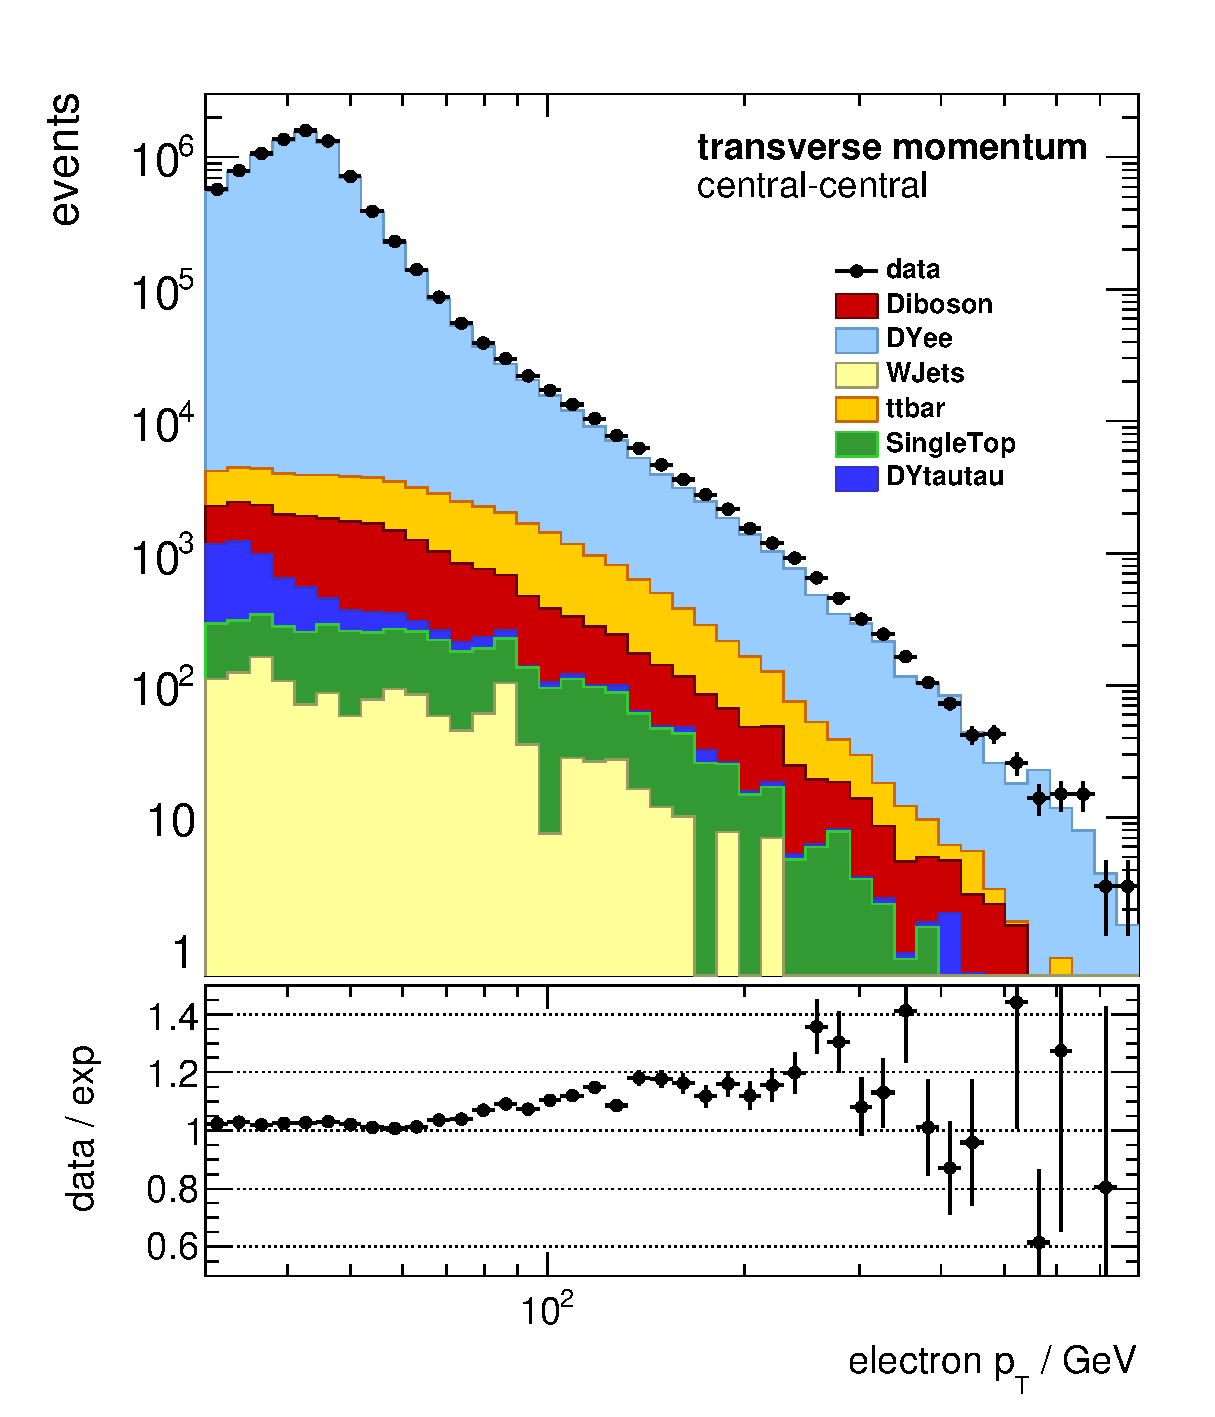
\includegraphics[width=0.48\textwidth]{plots/pt_cc}
    \hfill
    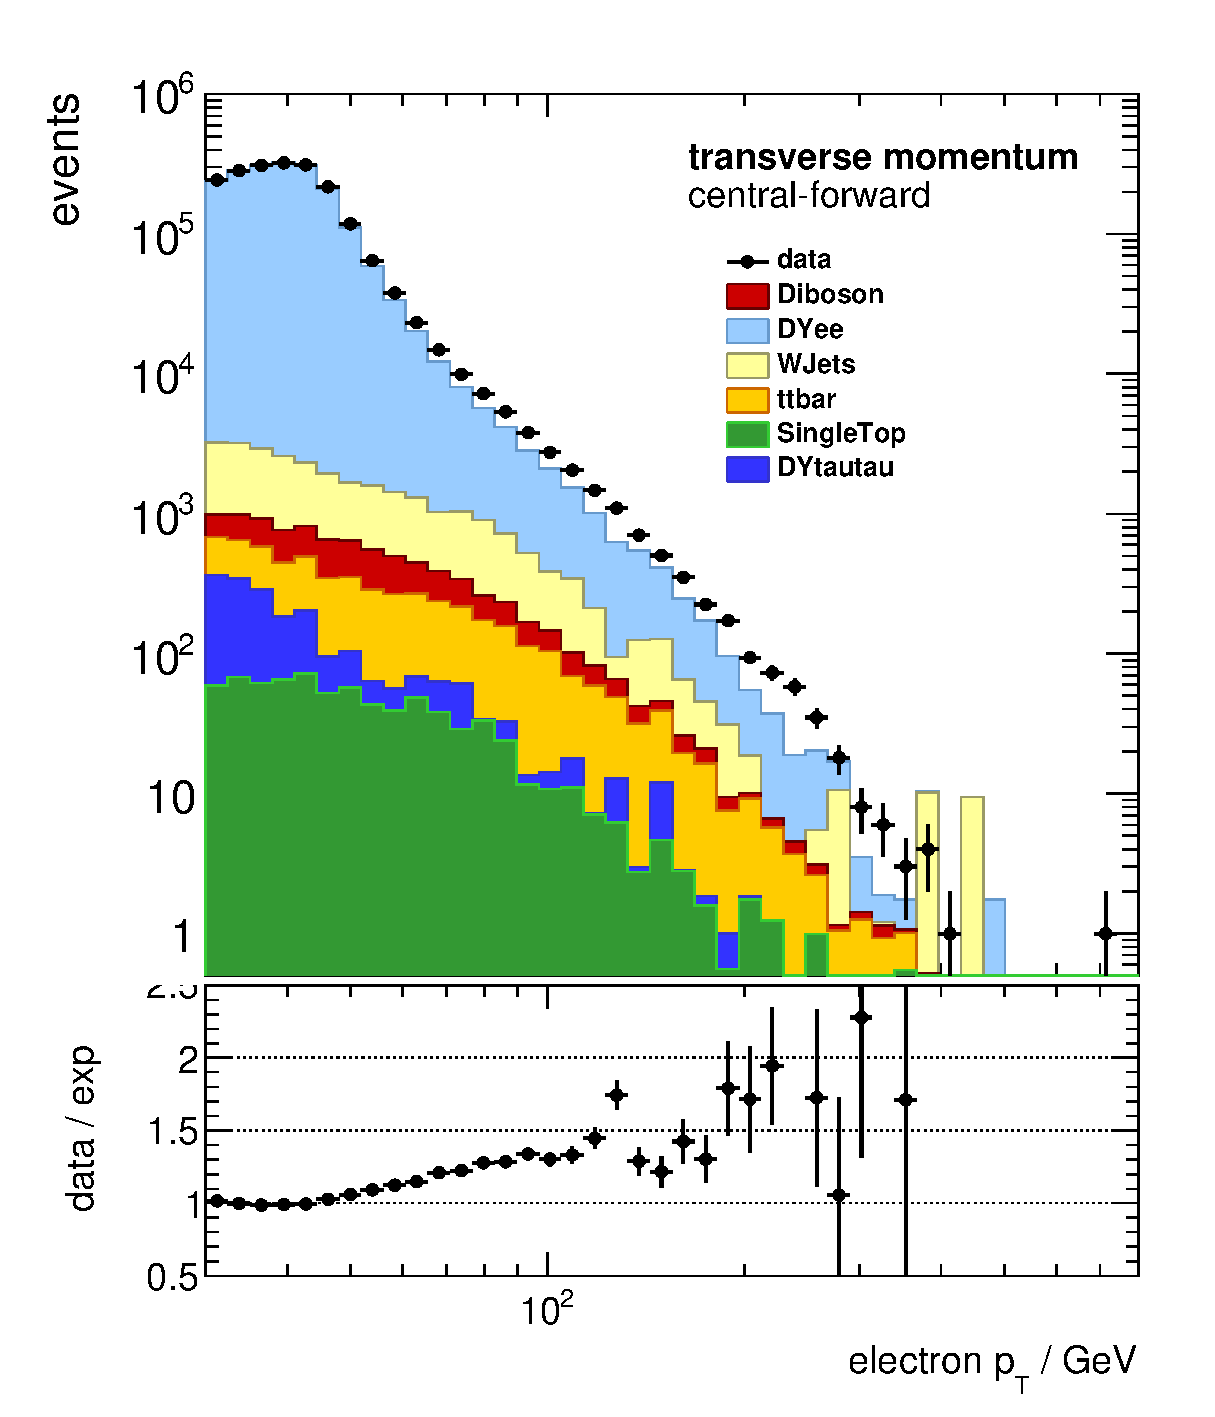
\includegraphics[width=0.48\textwidth]{plots/pt_cf}

    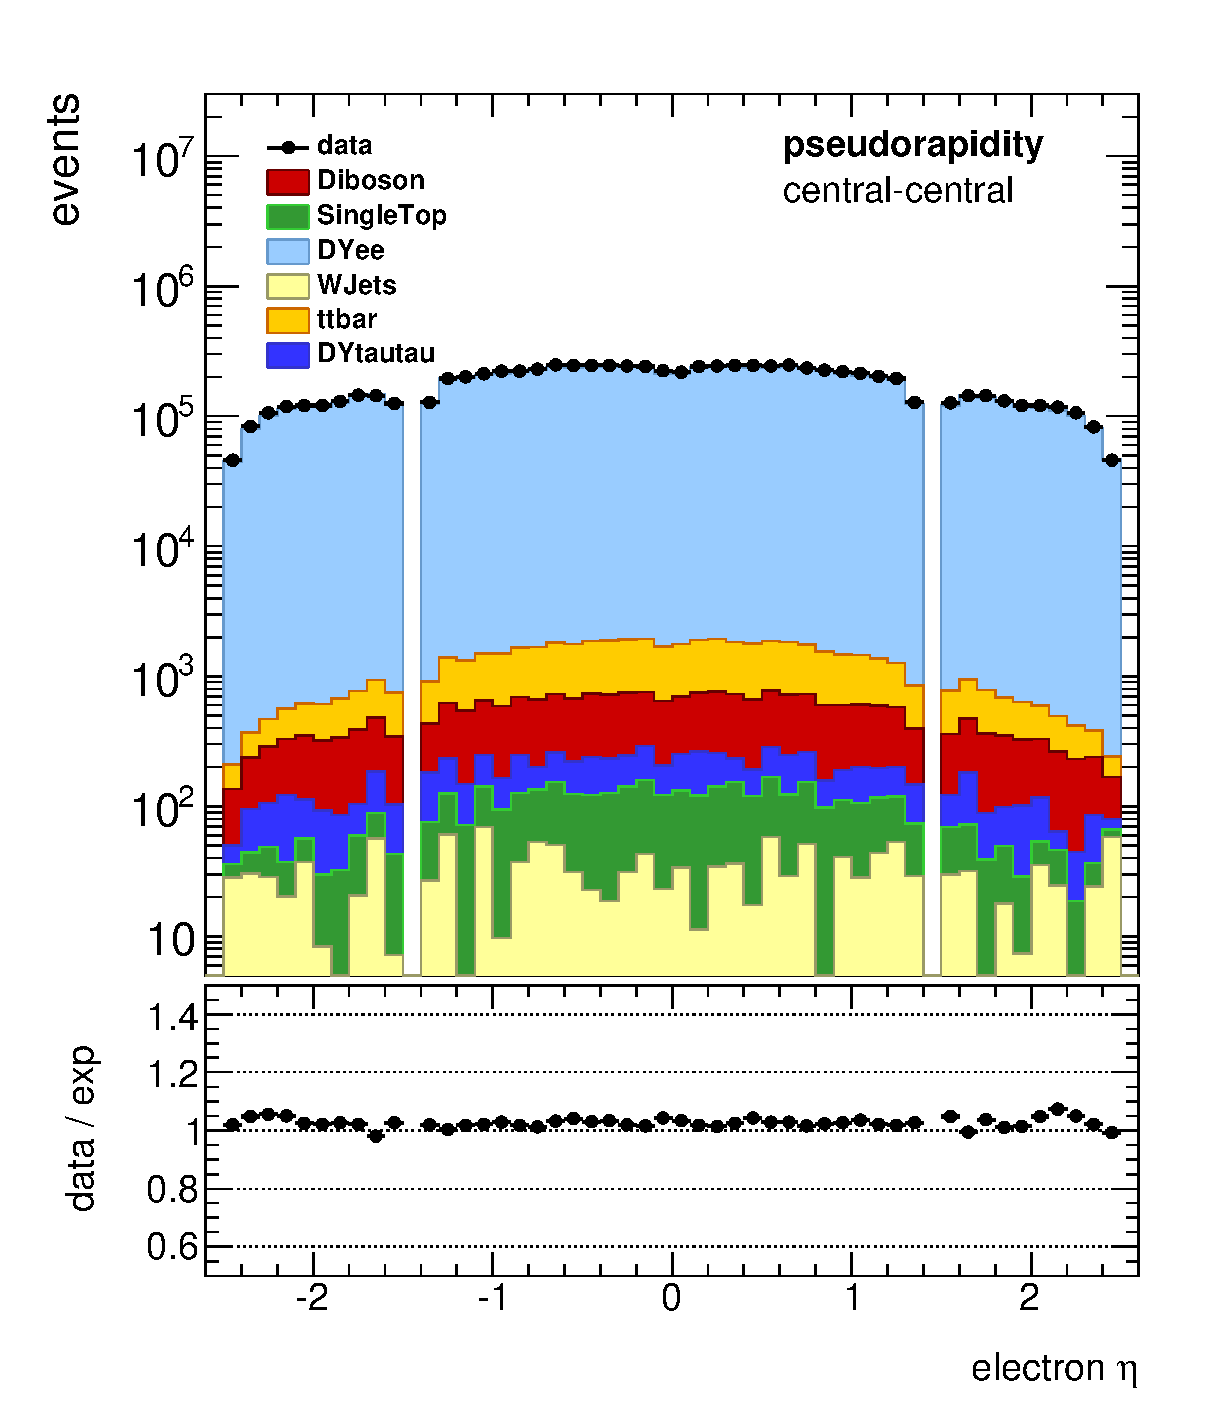
\includegraphics[width=0.48\textwidth]{plots/eta_cc}
    \hfill
    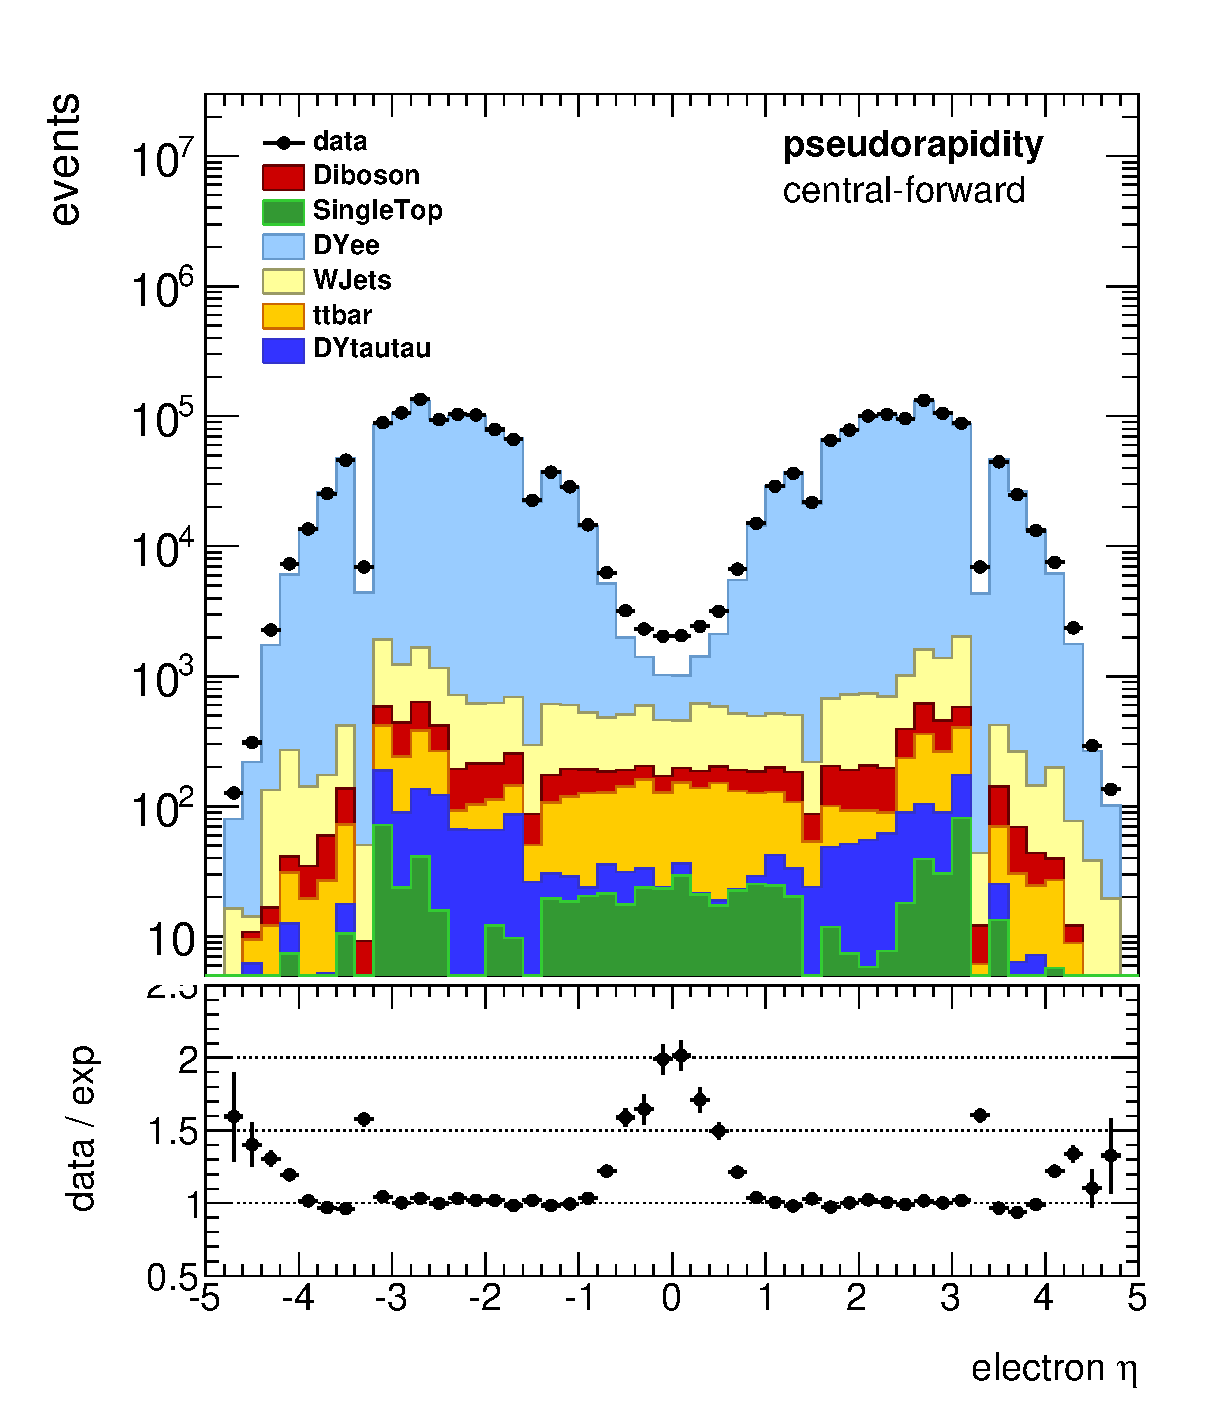
\includegraphics[width=0.48\textwidth]{plots/eta_cf}
    \caption[Kinematische Verteilungen der Elektronen nach Selektion in \ac{CC}
        und \ac{CF}]
        {Kinematische Verteilungen der Elektronen nach Selektion in \ac{CC}
        (links) und \ac{CF} (rechts) für den Transversalimpuls (oben) und die
        Pseudorapidität (unten). Der Quotient aus Daten und dargestellter
        Untergundsumme ist jeweils unter den Histogrammen gezeigt.}
    \label{fig:elec_kinematics}
\end{figure}

Erwartungsgemäß zeigen die Verteilungen des Transversalimpulses in Daten ein
Maximum bei etwa $45\GeV$, also gerade der halben Masse des $Z$-Bosons
und einen daran anschließenden starken Abfall mit steigendem Transversalimpuls.
Ein analoges Verhalten wird bei der Simulation des Signalprozesses
(\texttt{DYee}) beobachtet. Die übrigen Untergrundspektren weisen ebenfalls den
erwarteten Verlauf eines mit größer werdendem $p_T$ abfallendes Spektrum auf,
zeigen dagegen aber keine ausgeprägte Extremstelle. Einzige Ausnahme dabei
stellt das \texttt{DYtautau} Spektrum dar, welches ein solches Maximum
unterhalb von $45\GeV$ aufweist. Die Verschiebung dieses Maximums unter die
halbe $Z$-Masse liegt darin begründet, dass die Elektronen in diesem Prozess
aus den direkten Zerfallsprodukten des Bosons, den Tauonen, hervorgehen und
folglich nicht deren vollen Impuls tragen.

Desweiteren fällt beim Vergleich zwischen den Spektren für \ac{CC}- und
\ac{CF}-Selektion auf, dass sich der Umfang der Untergrundbeiträge deutlich 
unterscheidet. Am deutlichsten zeigt sich dies beim \texttt{WJets}
Untergrund, der in \ac{CF} den größten Beitrag zum Untergrund darstellt,
während dessen Rolle in \ac{CC} von geringer Bedeutung ist. Die Ursache
hierfür ist, dass im Vorwärts-Bereich die Wahrscheinlichkeit der
Fehlidentifikation eines Jets als Elektron wesentlich höher ist, als im
Zentral-Bereich, was unter anderem auf die fehlende Spurinformation im
Vorwärts-Bereich zurückzuführen ist\footnote{siehe hierzu auch Kapitel \ref{}}.

Unter jeder Abbildung ist zudem der Quotient aus der Datenverteilung und der
Summe alle Monte-Carlos (Untergründe + Signal) dargestellt. Diese zeigt, gerade
in Bereichen mit hohem Transversalimpuls eine deutliche Diskrepanz. Hierin
verbirgt sich ein weiterer bisher nicht betrachteter Untergundbeitrag der durch
Prozesse der \ac{QCD} bestimmt ist und deshalb nur schwer simulierbar ist. Die
Methode zur Abschätzung dieses Beitrags ist Gegenstand des nachfolgenden
Abschnitts.

Bei der Betrachtung der Spektren der Pseudorapidität ist zunächst zu beachten,
dass diese auf unterschiedlichen Skalen, entsprechend der jeweiligen Schnitte
in der Selektion, aufgetragen sind. In beiden Selektionen zeigen sich
natürlicherweise um Null symmetrische Spektren und die Exklusionen der
Kalorimeter Übergangsregionen ist deutlich sichtbar. Die Form der Verteilungen
im \ac{CC} Kanal zeigen einen leicht nach außen abfallenden Verlauf, während im
\ac{CF} Kanal zwei deutliche Erhebungen auszumachen sind. Diese haben ihr
Maximum bei $\eta\approx\pm 2,5$, was dem Übergang zwischen Zentral- und
Vorwärts-Bereich entspricht. Die Ausprägung dieser Struktur ist den
angewendeten Selektionkriterien geschuldet, die den Öffnungswinkel
zwischen den beiden Elektronen in der \ac{CF}-Selektion
einschränken\footnote{die \ac{CF} Selektion unterdrückt Ereignisse mit
Öffnungswinkeln $\theta \approx \pi$}. Die Untergrundbeiträge tragen hier
selbstverständlich im gleichen Maße bei, wie schon bei den Spektren des
Transversalimpulses erläutert. Schaut auf den jeweils darunter dargestellten
Quotienten aus Daten und Monte-Carlo, lässt sich etwas über den bisher
vernachlässigten Beitrag des \ac{QCD} Untergrundes etwas lernen. So resultiert
dessen Ignorieren im \ac{CC}-Kanal zu einem breiten, den vollen $\eta$-Bereich
abdeckenden Überschuss an Datenereignissen, während im \ac{CF}-Kanal diese
Überschüsse auf die Randbereiche ($|\eta| > 4,0$) und um das Zentrum ($\eta=0$)
konzentrieren.



\subsection{Datengestützte Untergrundabschätzung}
\label{afb:multijet}
Nachdem im vorangegangenen Abschnitt die Untergrundbeiträge simulierbarer
Prozesse untersucht wurden, steht nun die Examinierung der eben bereits
erwähnten Beiträge durch reine Prozesse der starken Wechselwirkung an. Die
Anzahl der möglichen Parton-Konstellationen innerhalb dieser Prozesse ist groß,
jedoch ist allen beitragenden Ereignissen gemein, dass sie mindestens zwei Jets
im Endzustand aufweisen, die irrtümlich als Elektronen rekonstruiert werden,
weshalb im Folgenden auch von \texttt{MultiJet} Untergrund gesprochen wird.

Zu dessen Abschätzung wird die sogenannte \textit{ReverseID}-Methode (vom engl.
reverse, umgekehrt) benutzt. Das Grundprinzip dabei sieht vor, einen neuen Satz
von Selektionsschnitten zu erstellen, der sich gegenüber der normalen
Signalselektion lediglich in der Umkehrung der Identifiaktionskriterien
unterscheidet. Das heißt konkret man verlangt anstelle einer bestimmten
Identifikationsstufe\footnote{z.B. \textit{tight++} (siehe Kapitel
\ref{})} für Elektronkandidaten die darunter liegende Stufe und fordert
gleichzeitig das Scheitern des ursprünglichen Kriteriums. Abbildung
\ref{fig:reverseID} veranschaulicht dies.
\begin{figure}[h]
    \centering
    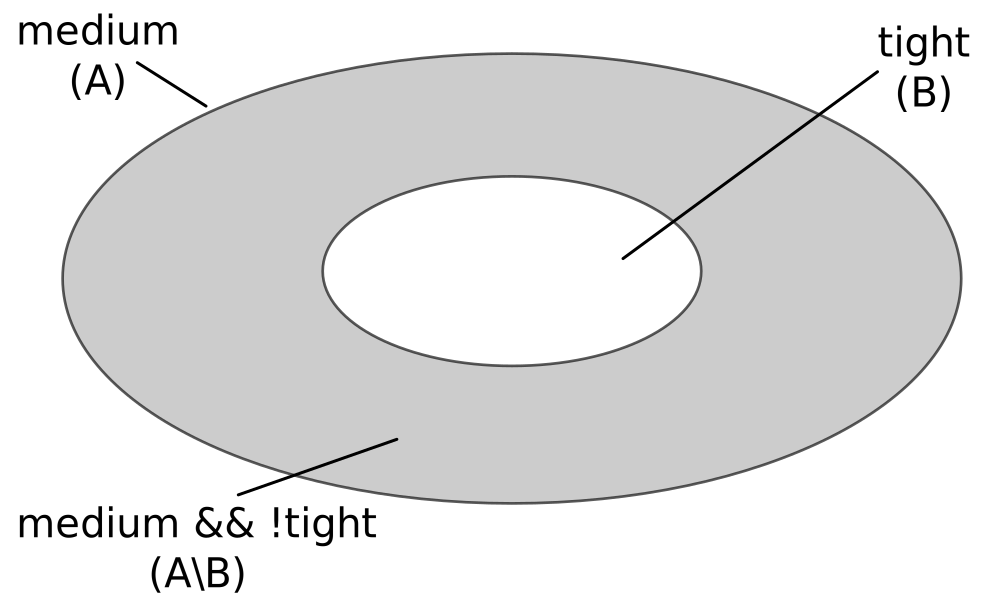
\includegraphics[width=0.5\textwidth]{img/reverseID}
    \caption[Mengentheoretische Darstellung der Selektion in der
        ReverseID-Methode]
        {Mengentheoretische Darstellung der Selektion in der ReverseID-Methode.
        \textbf{Signalselektion:} $B\quad$ \textbf{ReverseID-Selektion:}
        $A \backslash B$}
    \label{fig:reverseID}
\end{figure}
Da die Menge der Elektronen, die eine bestimmte ID-Stufe erfüllen stets eine
Teilmenge der darunterliegenden Stufe ist, ist die Menge der mit ReverseID
selektierten Elektronen statistisch unabhängig von der ursprünglichen Menge.
Auf den vollen Datensatz angewendet ist das Ziel dabei die Auslese jener
Ereignisse mit signalähnlichen Jets, die eine hohe Wahrscheinlichkeit haben als
Elektronen identifiziert zu werden.

Man trifft nun die Annahme, dass die statistische Verteilung dieser Ereignisse
geeignet ist, um die Form des \texttt{MultiJet} Untergrundbeitrages zu
repräsentieren, lediglich die Skalierung bleibt noch zu bestimmen. Letzteres
wird erreicht, indem man alle simulierten Untergünde (s.o.), das Signal
Monte-Carlo und die \texttt{MultiJet} Verteilung aufaddiert und diese Summe
mittels eines freien Skalierungsfaktors für die \texttt{MultiJet} Verteilung an
die beobachtete Datenverteilung anpasst.

Um Doppelzählungen mit fehlrekonstruierten Jets aus bereits simulierten
Untergründen (siehe voheriger Abschnitt) auszuschließen wird die ReverseID
Selektion ebenfalls auf alle bereits verwendeten Monte-Carlos angewandt und
deren Beitrag von der aus Daten erzeugten Verteilung subtrahiert.

In dieser Arbeit wird für die Signalselektion die Identifikationsstufe
\textit{tight++} für Zentral- bzw. \textit{fwdTight} für Vorwärts-Elektronen
verwendet. Dementsprechend werden für die ReverseID-Methode die folgenden
ID-Kriterien gefordert:
\begin{table}[h]
    \centering
    \begin{tabular}{
                        |c|
                        >{\centering\arraybackslash}p{45mm} |
                        >{\centering\arraybackslash}p{45mm} |
                   }
        \hline
        \bf{Bereich} & \bf{Signal Selektion} & \bf{ReverseID Selektion} \\
        \hline\hline
        Zentral  & \it{tight++}  & \textit{medium++} $\wedge$!\it{tight++} \\
        \hline
        Vorwärts & \it{fwdTight} & \textit{fwdMedium} $\wedge$!\it{fwdTight} \\
        \hline
    \end{tabular}
    \caption[Identifikations Kriterien der ReverseID-Methode]
        {Identifikations Kriterien der ReverseID-Methode. Ein '!' meint eine
        logische Negierung.}
    \label{tab:reverseID}
\end{table}

Zur Bestimmung des Skalierungsfaktors wird das, bereits für die
Kurvenanpassungen der Energiekalibration verwendete, Software-Paket
\textsc{RooFit} (\cite{Verkerke:2003ir}) verwendet. Dieses stellt die
Möglichkeit bereit Histogramme als Anpassungsmodelle zu verwenden. Oben
definierte \texttt{MultiJet} Verteilung wird nun als solches Modell mittels des
freien Skalierungsfakotrs an die Datenverteilung angepasst.

Abbildung \ref{fig:multijet} zeigt das Ergebnis dieser Anpassung im invarianten
Massenspektrum der Elektronpaare für den \ac{CC} und \ac{CF} Kanal.
\begin{figure}[h]
    \centering
    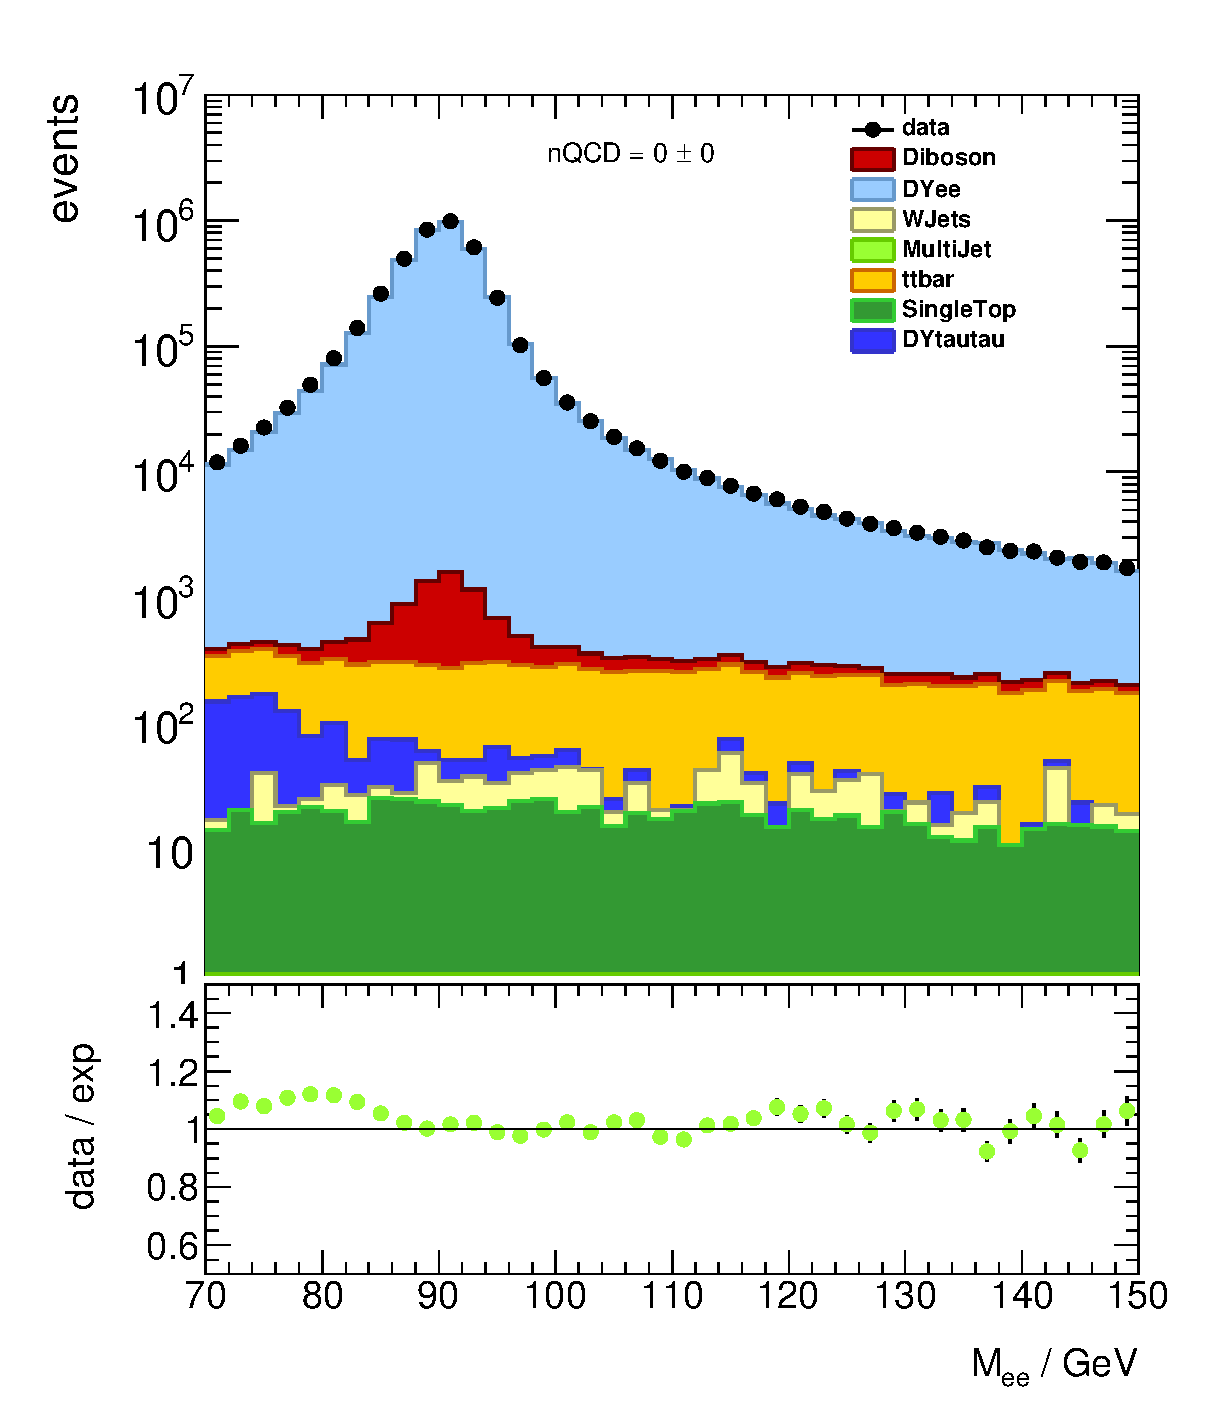
\includegraphics[width=.48\textwidth]{plots/mee_cc}
    \hfill
    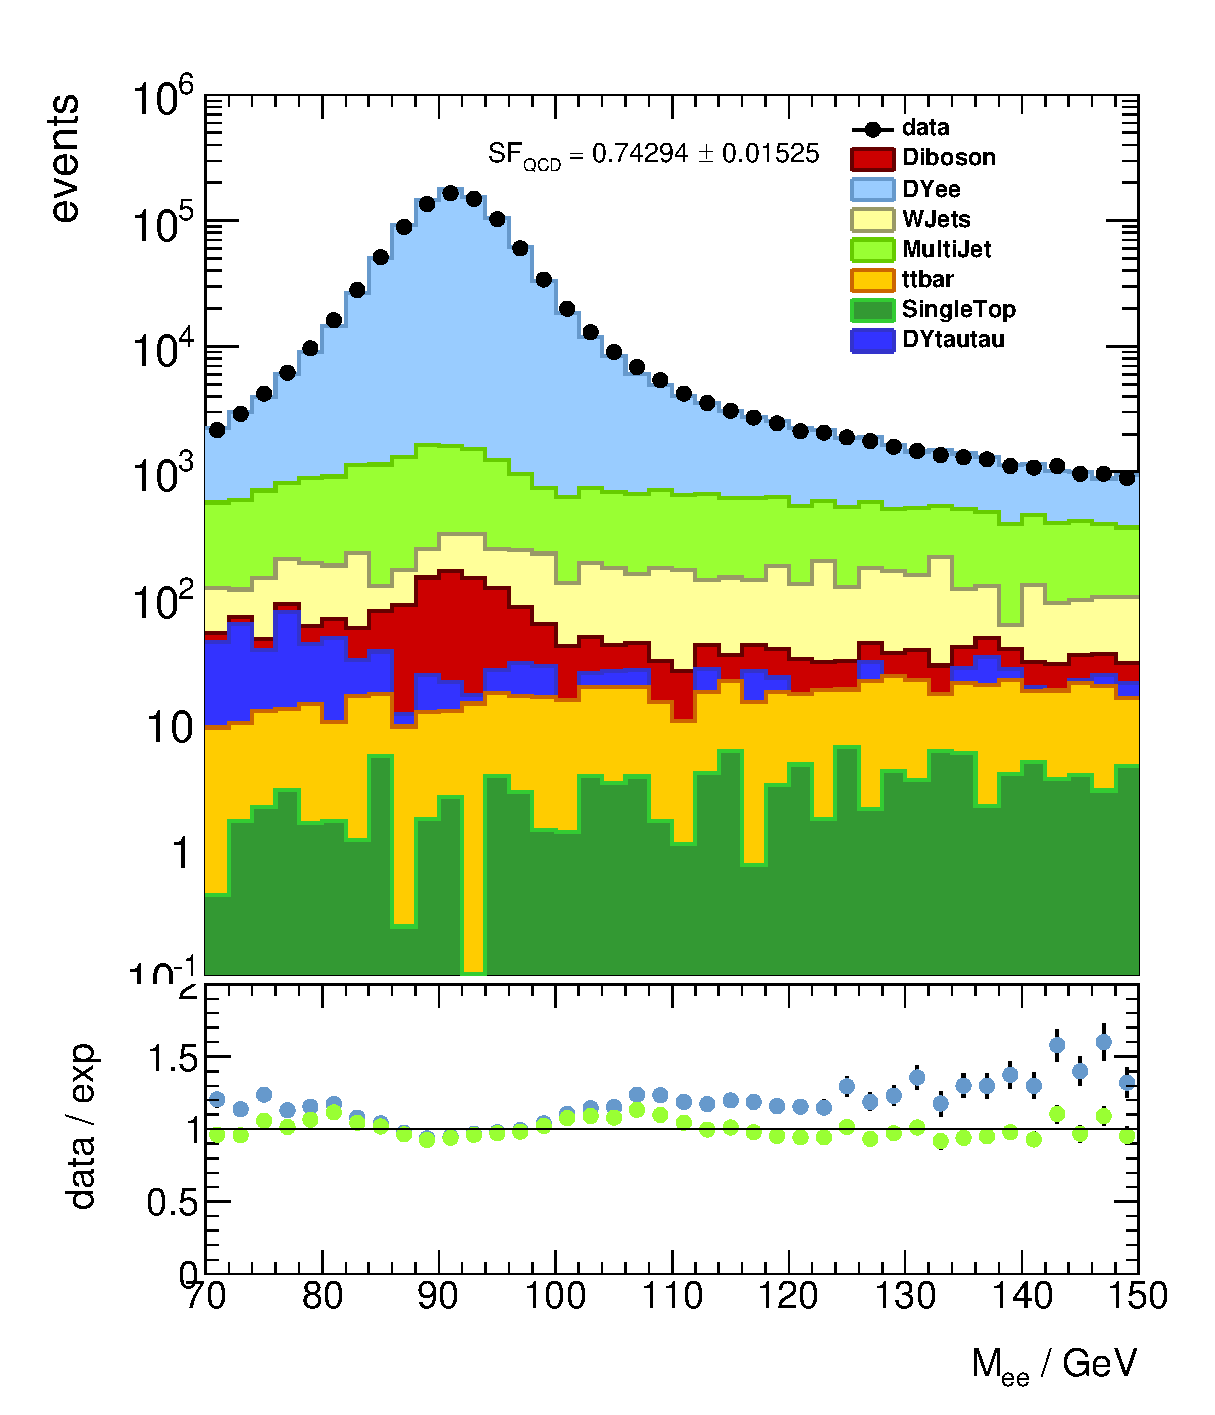
\includegraphics[width=.48\textwidth]{plots/mee_cf}
    \caption[Invariante Masse der Elektronpaare nach MultiJet
        Untergrundanpassung]
        {Invariante Masse der Elektronpaare mit MultiJet Untergrundanpassung
        und allen simulierten Untergründen im \ac{CC}-Kanal (links) und
        \ac{CF}-Kanal (rechts). Die darunter dargestellten Quotienten aus Daten
        und Summe aller Untergründe mit Signal Monte-Carlo zeigen die
        Übereinstimmung vor (blau) und nach (grün) MultiJet-Anpassung.}
    \label{fig:multijet}
\end{figure}
Dabei ist zunächst zu beachten, dass der Bereich der invarianten Masse auf
$70\GeV < M_{ee} < 150\GeV$ eingeschränkt wurde,was zwei Gründe hat. Zum einen
wurde diese Einschränkung schon im Hinblick auf die spätere Extraktion des
schwachen Mischungswinkels vorgenommen und zum anderen weißt die
ReverseID-Methode in höheren Massenbereichen signifkante Defizite auf, welche
deren Anwengung nicht mehr rechtfertigen lassen. So ist zum Beispiel die stetig
abnehmende Statistik ein Problem, viel mehr jedoch die unhaltbare Annahme Jets
würden sich über alle Energien und Bereiche des Detektors stets gleich
verhalten. Alternative Möglichkeiten zur Abschätzung der \ac{QCD}
Untergrundbeiträge werden am Ende des Kapitel diskutiert werden.

Die ermittelten Skalenfaktoren für beide Kanäle sind in Abbildung
\ref{fig:multijet} selbst dargestellt. Im \ac{CF}-Kanal, für den ein großer
Beitrag von \ac{QCD} Ereignissen erwartet wird, zeigt sich dieser mit einem
großen Anteil am Untegrundspektrum. Die Form der \texttt{MultiJet} Verteilung
ist ebenfalls gemäß der Erwartung durchweg flach. Die unter der Verteilung
dargestellten Verhältnisse von Daten zur Summe aller Untergründe und
Signal Monte-Carlo zeigt eine deutliche Verbesserung der Übereinstimmung unter
Hinzunahme des \texttt{MultiJet} Untergrundes. Für den \ac{CC} Kanal zeigt
sich, dass der Beitrag durch \ac{QCD} Ereignisse vernachlässigbar klein
gegenüber alle anderen Untergründen ist, sodass hier kein von Null
verschiedener Faktor ermittelt werden konnte. Die Betrachtung des Verhältnisses
darunter zeigt auch bereits eine hinreichend gute Übereintummung.  Einzig der
Bereich unterhalb von $80\GeV$ weist eine erhebliche Abweichung auf, welches
aber auf ein bekanntes Problem mit der Detektor-Beschreibung innerhalb der
Monte-Carlo Simulation zurückführen ist, welches derzeit von der zuständigen
ATLAS Arbeitsgruppe untersucht wird.



%______________________________________________________________________________
%                            Winkelverteilung und Vorwärts-Rückwärts Asymmetrie
\section{Winkelverteilung und Vorwärts-Rückwärts Asymmetrie}
\label{afb:afb}

% + Pythia Dilution Studie
% + Rohe Verteilung
% + Untergund reduzierte Verteilung
% + Vergleich mit Signal-Simulation

Nach der Abschätzung der Untergrundbeiträge folgt nun die Messung der
Vorwärts-Rückwärts Asymmetrie. Die relevanten Observablen hierbei sind die
invariante Masse $M_{ee}$ des Elektronpaares und der Emissionswinkel des
Elektrons definiert im Collins-Soper Bezugssystem $\cos\theta_{cs}$ (siehe
Gleichung (\ref{eq:collins_soper})). Letztere beinhaltet gegenüber der reinen
Definition (\ref{eq:collins_soper_raw}) den Vorzeichen bestimmenden
longitudinalen Impulsterm des Elektronpaares $p_z(e^+e^-)/|p_z(e^+e^-)|$,
welcher die Annahme über die Korrelation zwischen der ursprünglichen
Quarkrichtung und dem Lorentz-Boost des Elektronpaares wiederspiegelt. 



\subsection{Korrelation der Quark-Richtung mit dem Lorentz-Boost des Z-Bosons}
\label{afb:dilution}
Der Geltungsbereich dieser Annahme lässt sich mittels Monte-Carlo Simulationen
untersuchen. Dazu werden mit dem Monte-Carlo Generator \textsc{Pythia8}
(\cite{Sjostrand:2007gs}) für unterschiedliche Bereiche in der invarianten
Masse Ereignisse simuliert. Eine anschließende Detektor-Simulation findet nicht
statt\footnote{Die Simulation der Detektor-Antwort ist für die angestrebte
Untersuchung irrelevant}. Da der Generator die volle kinematische Information
der im Prozess beteiligten Partonen zur Verfügung stellt, lässt sich ein
Vergleich zwischen obigem Vorzeichen-Faktor und der originären Quarkrichtung
ziehen.

Die Simulation findet mit einer eigenständigen Installation\footnote{d.h. keine
von der ATLAS Monte-Carlo Workingroup verifizierte Simulation, was für den
angestrebten Zweck unnötig ist} von \textsc{Pythia8} statt deren
Konfiguration in Anhang \ref{pythia8:dilution} zu finden ist. Für insgesammt
sieben verschiedene Massenbereiche bis zu $1 \TeV$ wurden statistisch
unabhängige Datensätze von je $10$ Millionen Ereignissen generiert und jeweils
die Übereinstimmung zwischen der wahren Quark-Richtung und dem nach
$p_z(e^+e^-)/|p_z(e^+e^-)|$ Vorzeichen verglichen. Abbildung \ref{fig:dilution}
zeigt die resultierenden Verteilungen in Abhängigkeit vom Betrag der Rapidität
$|Y_{ee}|$ des Elektronpaares.

\begin{figure}[h]
    \centering
    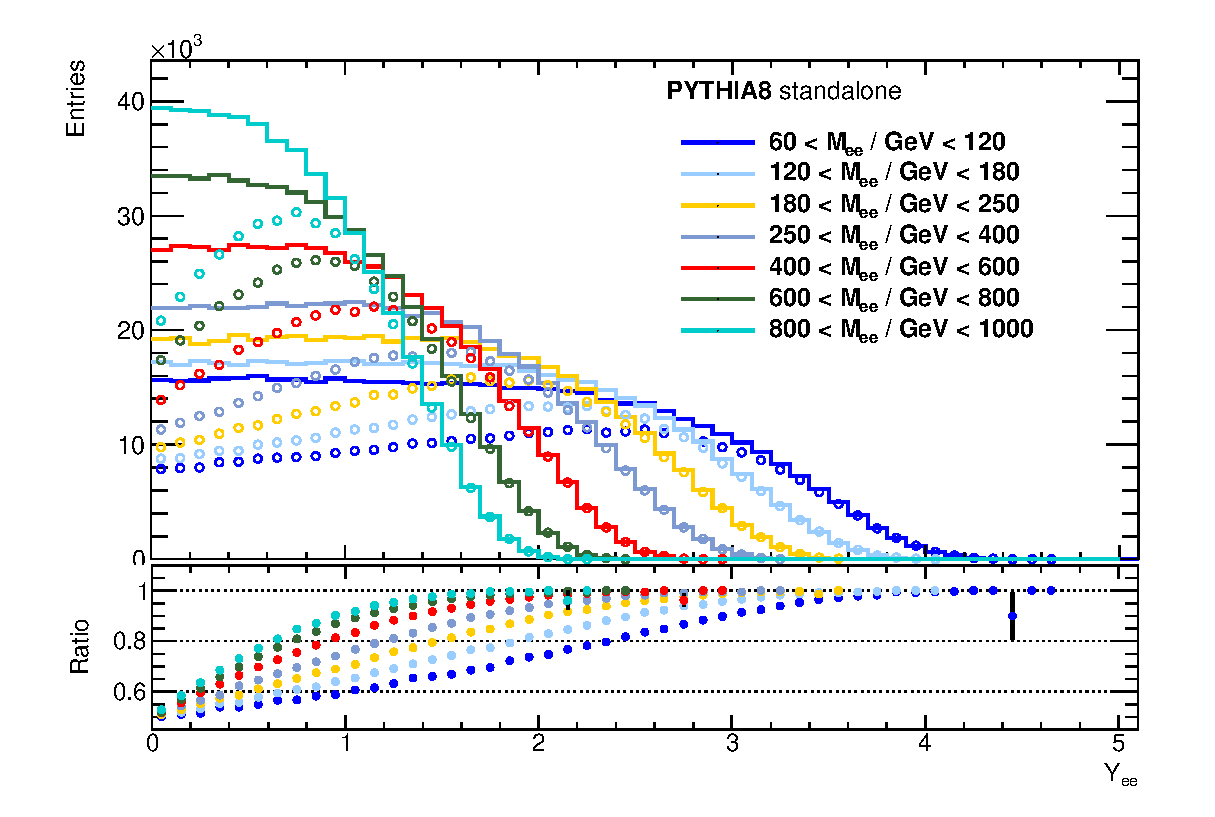
\includegraphics[width=0.6\textwidth]{plots/dilution}
    \caption[Vergleich zwischen Quark-Richtung und long. Komponente des
        Z-Boosts]
        {Vergleich zwischen wahrer Quark-Richtung und der longitudinal
        Komponente des Elektronpaar-Lorentzboosts. Die durchgezogenen
        Verteilungen beinhalten alle Elektronpaare, die Kreise nur solche mit
        korrekter Zuordnung der Quark-Richtung.}
    \label{fig:dilution}
\end{figure}

Für jeden Massenbereich sind zwei Verteilungen gezeigt. Mit einer
durchgezogenen Linie sind alle Elektronpaare repräsentiert, während die Kreise
all jene Elektronpaare mit korrekter Zuordnung der Quark-Richtung zeigen, d.h.
alle Paare für die gilt:
\begin{equation}
    p_z^q \cdot q_z^{e^+e^-} > 0
\end{equation}
Wie in jedem Massenbereich gut zu sehen ist nimmt die Übereinstimmung mit
größerem Betrag der Rapidität zu. Dies ist besonders eindrucksvoll an der
darunter gezeigten Verhältnissen zu sehen, die auch als
Wahrscheinlichkeitsverteilungen für die Fehlzuordnung der Quarkrichtung durch
die obige Annahme interpretiert werden können. Über alle Massenbereich hinweg
zeigt sich für Rapiditäten nahe bei Null eine Rate von $50\%$ für falsch
zugeordnete Quarkrichtungen, welche dann mit steigender Rapidität stetig
kleiner wird. Die Rate der korrekten Zuordnungen verbessert sich hingegen bei
konstanter Pseudorapidität mit steigender Masse, was sich in den
unterschiedlichen Steigungen der Verhältnisse wiederspiegelt.
 
Den Einfluss dieses Effekts auf die Messung der Asymmetrie im \ac{CC}- und
\ac{CF}-Kanal lässt sich am besten anhand der gemessenen Rapiditätsverteilungen
abschätzen. Diese sind in Abbildung \ref{fig:rapidities} gezeigt. Hier lässt
sich leich erkennen, dass die Ereignisse im \ac{CF}-Kanal vorwiegend die
Bereiche um $Y_{ee}=2,5$ populieren, während die Verteilung im \ac{CC}-Kanal
ihr Maximum bei $Y_{ee}=0$ zeigt, und dann nach außen hin abfällt.

\begin{figure}[h]
    \centering
    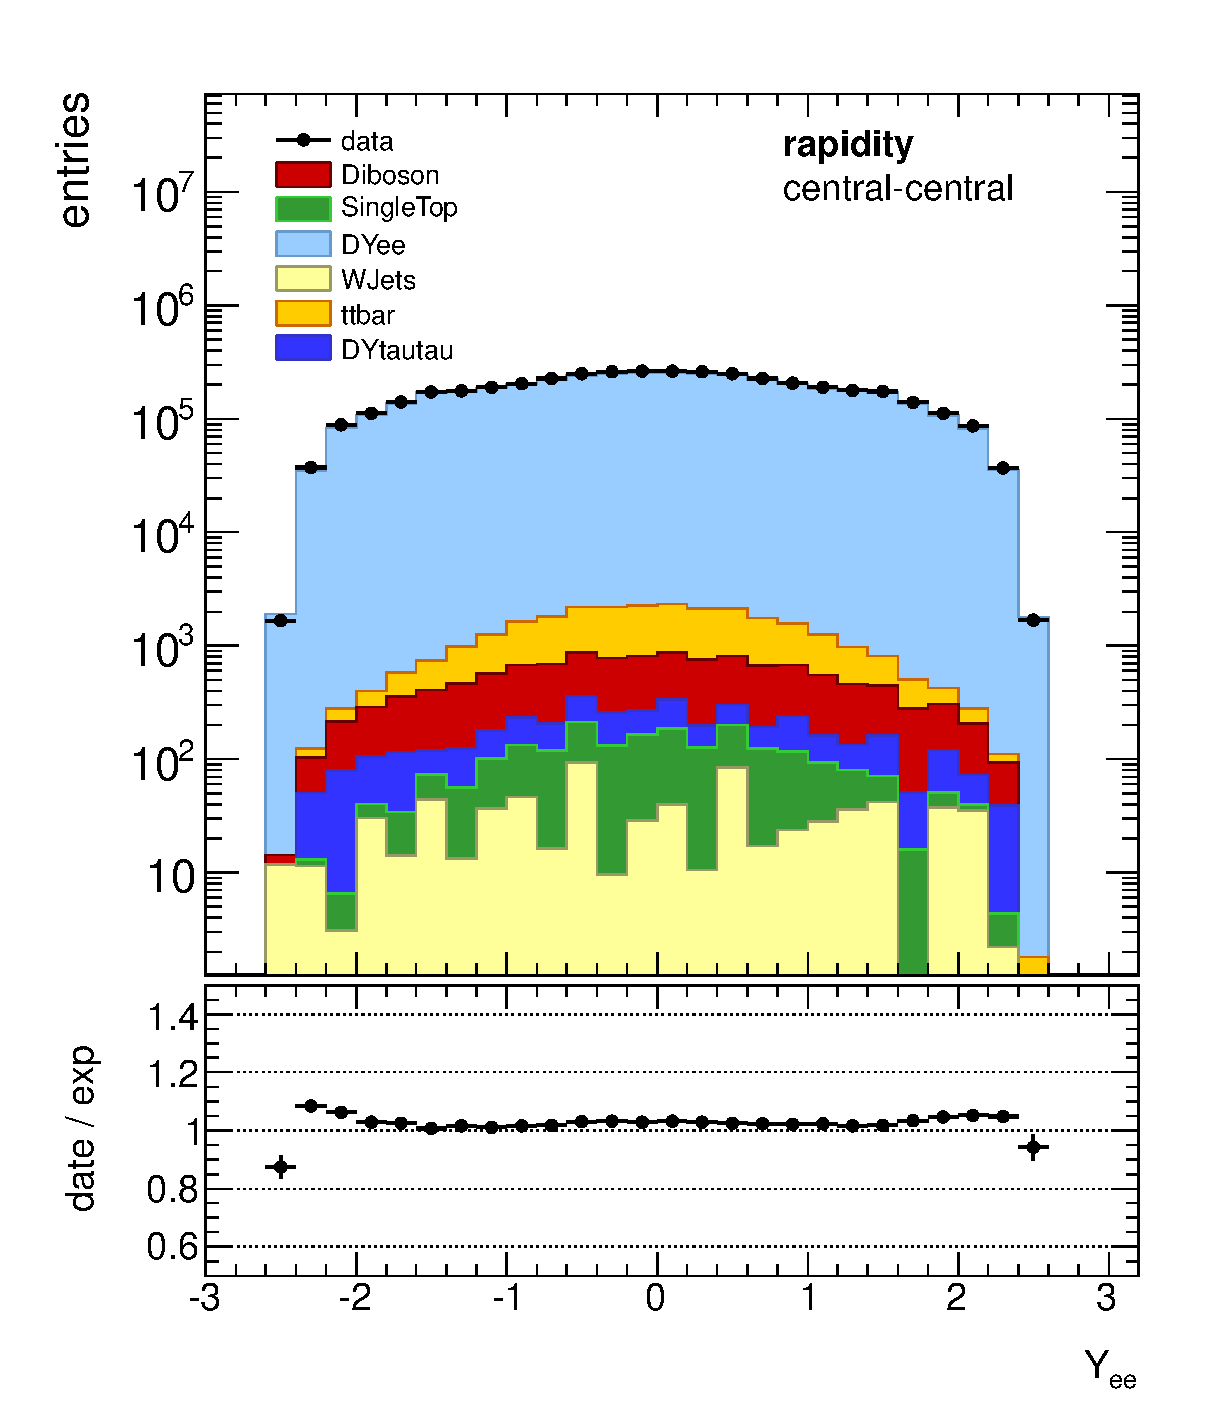
\includegraphics[width=0.48\textwidth]{plots/yee_cc}
    \hfill
    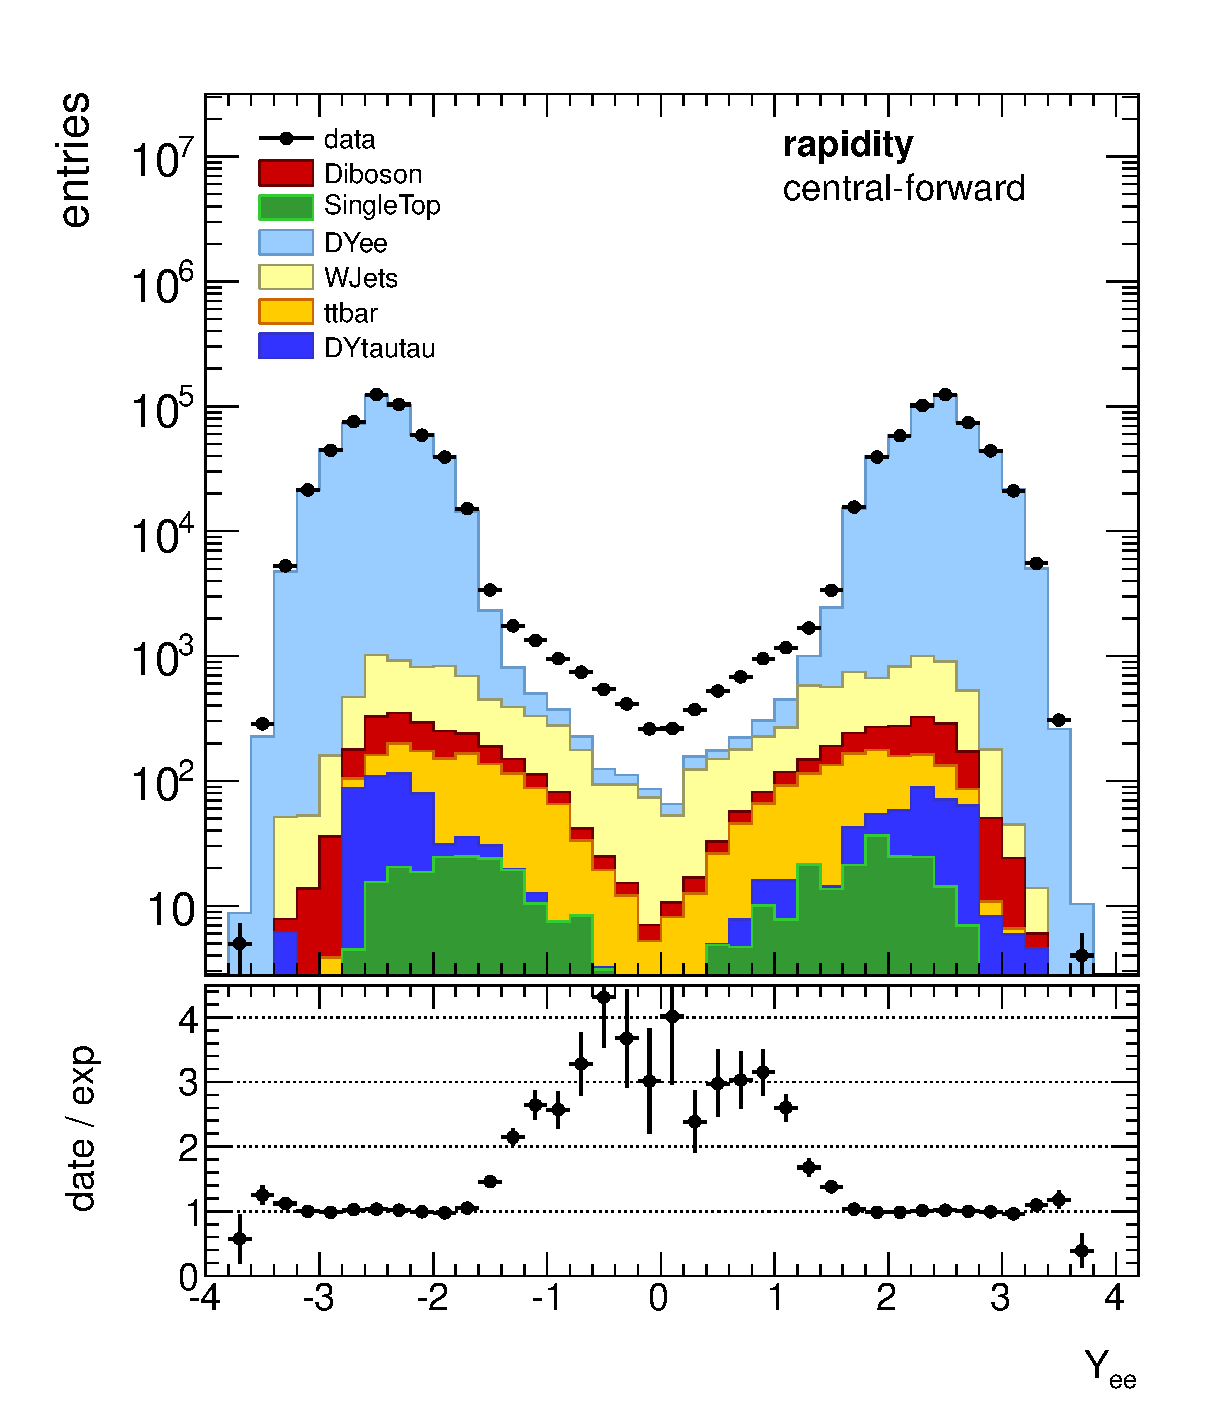
\includegraphics[width=0.48\textwidth]{plots/yee_cf}
    \caption[Rapiditäts-Verteilungen der Elektronpaare im \ac{CC}-Kanal
        und \ac{CF}-Kanal]
        {Rapiditäts-Verteilungen der Elektronpaare im \ac{CC}-Kanal
        (links) und \ac{CF}-Kanal (rechts) ohne \texttt{MultiJet}-Untergrund}
    \label{fig:rapidities}
\end{figure}

Alle falsch zugeordneten Ereignisse tragen mit zur Abschwächung (Dilution) der
Vorwärts-Rückwärts Asymmetrie bei, was sich somit vorwiegend im \ac{CC}-Kanal
bemerkbar machen sollte. Ein zusätzlicher Schnitt auf den Betrag der Rapidität
der Elektronpaare wäre denkbar, würde allerdings die Akzeptanz in hohem Maße
einschränken, sodass gerade im \ac{CC}-Kanal enorm an statistischer Signifikanz 
eingebüßt werden müsste. Deshalb wird in dieser Arbeit auf einen solchen
Schnitt verzichtet.



\subsection{Verteilungen der Vorwärts-Rückwärts Asymmetrie}
\label{afb:distributions}
Die Bestimmung der Vorwärts-Rückwärts Asymmetrie erfolgt für kleine Intervalle
der invarianten Masse der Elektronpaare aus der Differenz zwischen der Anzahl
vorwärts- und rückwärts-emittierter Elektronen normiert auf deren Gesamtzahl.
\begin{equation}
    \afb = \frac{N_F - N_B}{N_F + N_B}
    \label{eq:afb_simple}
\end{equation}
Wobei die Klassifizierung \textit{vorwärts} und \textit{rückwärts} nach dem
Vorzeichen von $\cos\theta_{cs}$ geschieht\footnote{siehe auch Gleichung
(\ref{eq:afb})}:
\begin{equation}
    \cos\theta_{cs} > 0 \quad\text{(vorwärts)}
    \qquad \qquad
    \cos\theta_{cs} < 0 \quad\text{(rückwärts)}
\end{equation}
Die Unterteilung in der invarianten Masse erfolgt in den gleichen Grenzen, wie
schon die Kurvenanpassungen der Energiekalibration der Vorwärts-Elektronen,
d.h. in einem Fenster um die Z-Resonanz zwischen $75\GeV$ und $105\GeV$. Die
Aufteilung findet prinzipiell in Schritten von $2\GeV$ statt, wobei die
statistisch weniger polpulierten Randbreiche in größeren Abständen unterteilt
werden. Die folgende Tabelle \ref{tab:binning_afb} zeigt die gewählte
Einteilung über den Massenbereich.
\begin{table}[h]
    \centering
    \begin{tabular}{|c|c|c|c|c|c|c|c|c|c|c|c|}
        \multicolumn{12}{c}{\textbf{Invariante Masse} [$\GeV\:$]} \\
        \hline
        $75,0$ & $80,0$ & $83,0$ & $85,0$ & $87,0$ & $89,0$ & $91,0$ & $93,0$ &
        $95,0$ & $97,0$ & $100,0$ & $105,0$
        \\ \hline
    \end{tabular}
    \caption[Unterteilung in der invarianten Masse des Elektronpaares zur
        Bestimmung der Vorwärts-Rückwärts Asymmetrie]
        {Unterteilung in der invarianten Masse des Elektronpaares zur
        Bestimmung der Vorwärts-Rückwärts Asymmetrie}
    \label{tab:binning_afb}
\end{table}

Zur Berechnung der Vorwärts-Rückwärts Asymmetrie werden nun die Daten,
Untegründe und die Signal-Simulation nach oben beschriebener Selektion
(Abschnitt \ref{afb:selection}) und ggf. Anwendung der Korrekturen in je zwei
Histogramme der invarianten Masse aufgeteilt. Eines mit Ereingissen
vorwärts-emittierter Elektronen und eines mit Ereignissen rückwärts-emittierter
Elektronen. Von beiden Verteilungen der realen Daten werden anschließend die
entsprechenden Histogramme aller Untergründe subtrahiert. Die Berechnung der
Asymmetrie nach Gleichung (\ref{eq:afb_simple}) geschieht dann für die
untergrund-reduzierten Daten und das Signal Monte-Carlo in jedem Bereich der
invarianten Masse (Tabelle \ref{tab:binning_afb}) separat. Abbildung
\ref{fig:afb_raw} zeigt die resultierenden Asymmetrie-Verteilungen für die
beiden Selektionskanäle \ac{CC} und \ac{CF}.

\begin{figure}
    \centering
    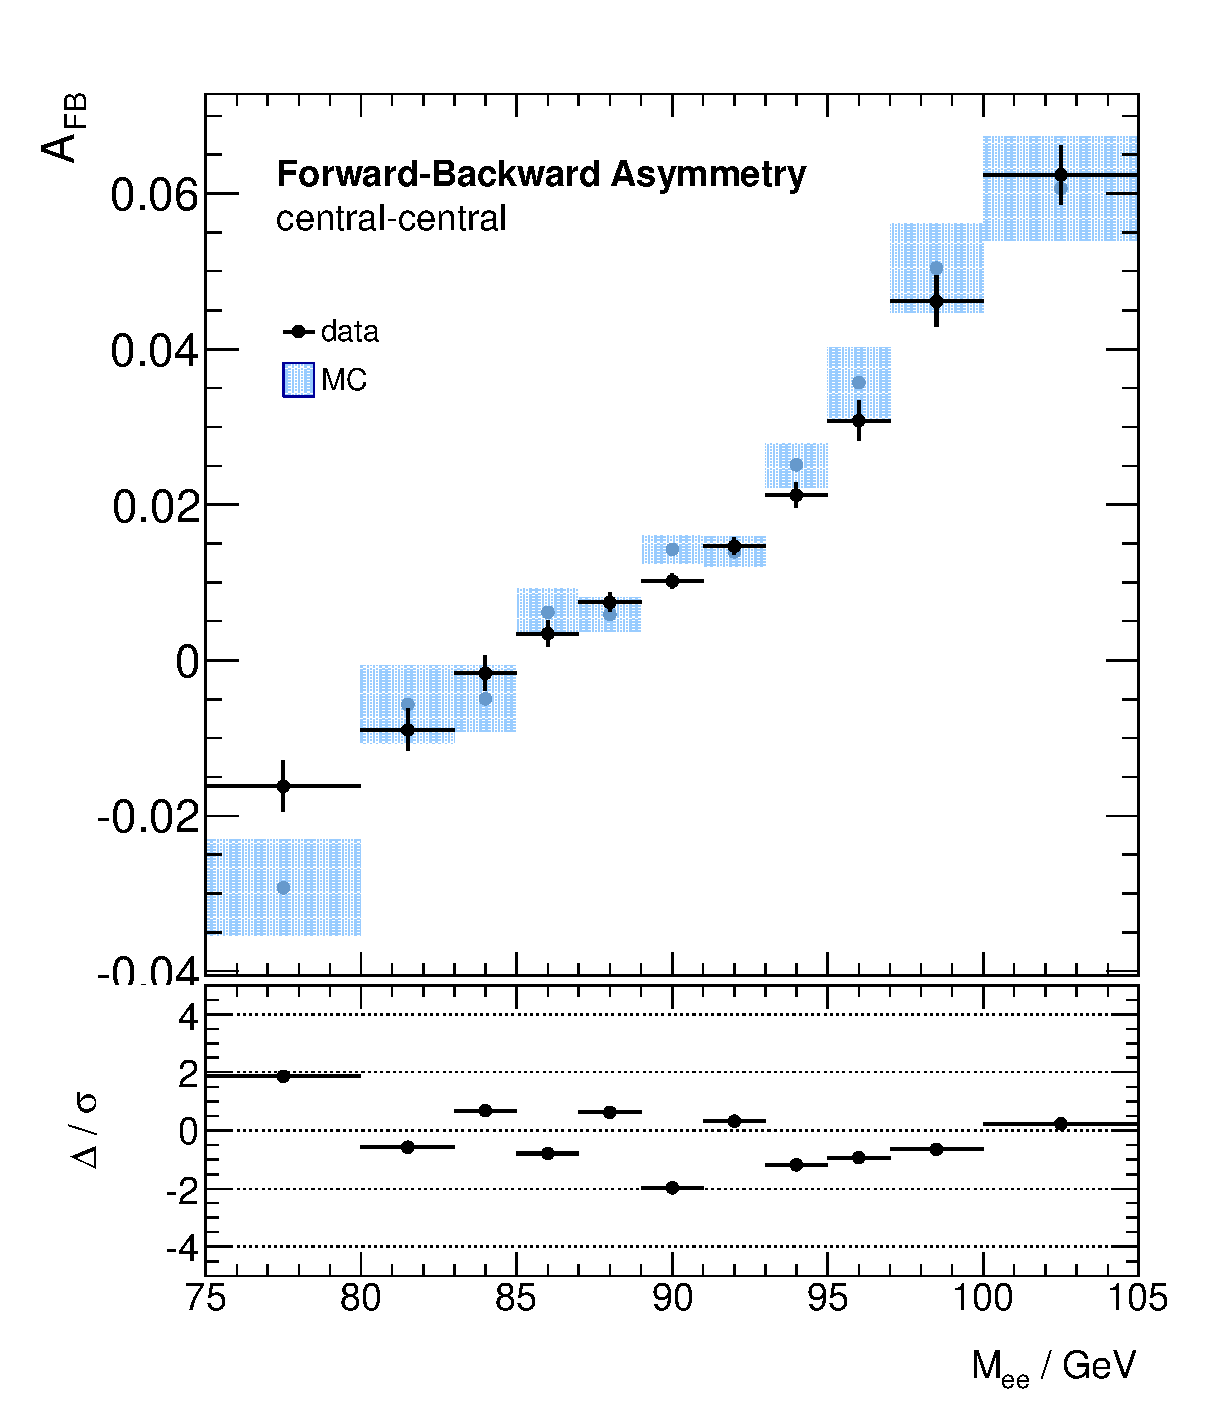
\includegraphics[width=0.48\textwidth]{plots/afb_cc}
    \hfill
    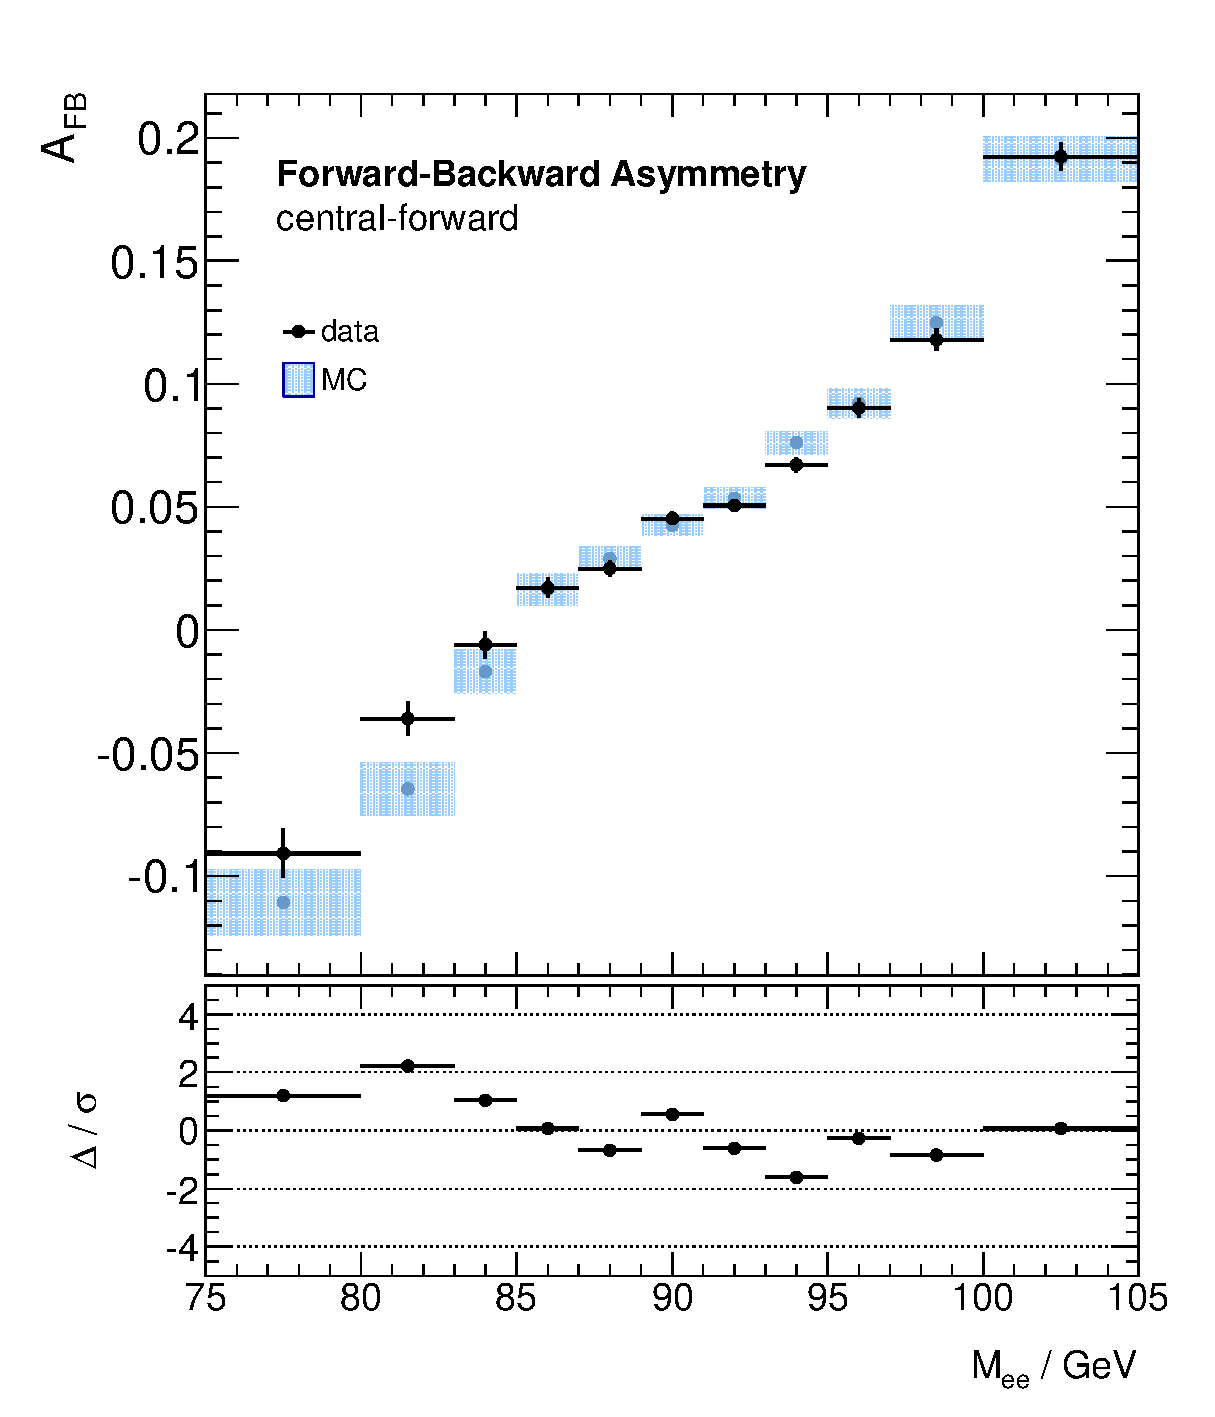
\includegraphics[width=0.48\textwidth]{plots/afb_cf}
    \caption[Verteilung der Vorwärts-Rückwärts Asymmetrie im \ac{CC}-Kanal
        und \ac{CF}-Kanal]
        {Verteilung der Vorwärts-Rückwärts Asymmetrie im \ac{CC}-Kanal
        (links) und \ac{CF}-Kanal (rechts) um die Z-Resonanz. (Nur statistische
        Unsicherheiten)}
    \label{fig:afb_raw}
\end{figure}

In der Verteilung der Daten zeigt sich die erwartete Form der
Asymmetrie\footnote{vgl. Abbildung \ref{}}, wobei zunächst auffällt, dass diese
im \ac{CF}-Kanal sehr viel stärker ausgeprägt ist, als im \ac{CC}-Kanal. Die
Skalierung der Ordinate macht dies deutlich. Die Ursache dafür liegt in der
bereits in Abschnitt \ref{afb:dilution} diskutierten höheren Wahrscheinlichkeit
einer falschen Zuordnung der Quark-Richtung für Ereignisse mit niedriger
Rapidität $Y_{ee}$ des Elektronpaares\footnote{Die Verteilungen der Rapiditäten
sind in Abbildung \ref{fig:rapidities} gezeigt}, was zu einer Abschwächung der
Asymmetrie führt.

Desweiteren zeigt sich in beiden Kanälen, jedoch prominenter im \ac{CF}-Kanal
zu beobachten, dass die Steigung der Asymmetrie sehr nahe an der Z-Resonanz
kleiner ist, als in den Bereichen darunter und darüber. Die theoretische Form
der Verteilung (Abbildung \ref{}) weist disen Effekt hingegen nicht auf. Da
dieses Verhalten allerdings auch im Signal Monte-Carlo zu beobachten ist, liegt
die Vermutung nahe, dass die endliche Massenauflösung des Detektors dafür
verantwortlich ist. So wird später bei der Erstellung der Form-Vorlagen zur
Extraktion des schwachen Mischungswinkels die Einführung von Detektoreffekten
in die Theorie-Verteilungen zum gleichen Effekt führen (siehe nachfolgenden
Abschnitt \ref{afb:extraction_method}).

Unterhalb der Asymmetrie-Verteilungen ist die Differenz zwischen der aus Daten
gewonnen Verteilung und dem Singal Monte-Carlo in Einheiten der Standabweichung
gezeigt, wobei zu beachten ist, dass nur statistische Unsicherheiten erfasst
werden. Wie sich leicht erkennen lässt liegen die meisten Punkte innerhalb
einer $1\sigma$ Umgebung, was für eine gute Beschreibung der Daten durch die
Simulation spricht. Die signifkantesten Abweichungen jedoch zeigen sich in den
niedrigeren Bereichen der invarianten Masse, für die bereits in Abschnitt
\ref{afb:selection} belegt wurde, dass die Beschreibung der der Daten durch die
Untergründe und die Simulation nicht ausreichend gewährleistet ist.

Für die Untersuchung systematischer Einflüsse auf die Vorwärts-Rückwärts
Asymmtrie blieben im Rahmen dieser Arbeit keine Kapazitäten mehr, sodass deren
Bedeutung lediglich qualitativ diskutiert werden kann. Da die Asymmetrie aus
dem Quotienten (\ref{eq:afb_simple}) hervorgeht, spielen Einflüsse, welche die
Ereignismengen $N_F$ und $N_B$ gleichermaßen skalieren, keine Rolle. Dagegen 
tragen Variationen, die die Zugehörigkeit von Ereignissen zu einer oder der
anderen Menge ändern, sogannte Migrations-Effekte, erhebliche Relevanz. In der
vorangegangenen Analyse der Vorwärts-Rückwärts Asymmetrie mit \acs{ATLAS}-Daten
des Vorjahres bei $7\TeV$ Schwerpunktsenergie (\cite{ATLAS-CONF-2013-043})
konnte gezeigt werden, dass die größten systematischen Unsicherheiten aus der
Energiekalibration der Elektronen\footnote{genauer die Unsicherheiten auf die
Kalibrationsfaktoren} und der Wahl der simulationsseitig zugrunde liegenden
\acl{PDF} resultieren. Beide Quellen sind in der Lage die Verteilung der
Asymmetrie sowohl zu verzerren, als auch zu verschieben. In wenig geringerem
Maße Einfluss nehmend sind die Unsicherheiten auf die Korrektur der
Energieauflösung, deren Zweck bereits die Migration von Ereignissen in der
invarianten Masse ist. Alle genannten Effekte lassen sich durch deren Variation
und der anschließenden Bestimmung der enstehenden Differenz zu obiger
Asymmetrie-Verteilung abschätzen.



%______________________________________________________________________________
%                          Extraktion des effektiven Schwachen Mischungswinkels
\section{Extraktion des effektiven Schwachen Mischungswinkels}
\label{afb:sin2theta}

Die Messung der Vorwärts-Rückwärts Asymmetrie ist die Grundlage für die
Extraktion des effektiven schwachen Mischungswinkels. Dessen Bestimmung findet
weiterhin in den Kanälen \ac{CC} und \ac{CF} getrennt statt, und wird erst am
Ende zu einem Gesamt-Ergebnis kombiniert. 



\subsection{Beschreibung der Extraktionsmethode}
\label{afb:extraction_method}

% + Extraktionsmethode
%   - Template Erzeugung
%   - Faltung mit Detektoreffekten
%   - Template zeigen (wg. Z-Resonanz AFB)

Zur Extraktion des effektiven schwachen Mischungswinkels aus den Verteilungen
der Vorwärts-Rückwärts Asymmetrie wird eine Vorlagen basierte Methode
verwendet. Die grundlegende Idee hierbei ist die Erstellung eines Satzes von
simulierten Asymmetrie-Verteilungen für verschiedene Werte des schwachen
Mischungswinkels und einem anchließenden $\chi^2$-Test, der die Übereinstimmung
jeder dieser Verteilungen mit der real in Daten beobachteten Verteilung
quantifiziert. Die resultierenden $\chi^2$-Werte aufgetragen gegen den
schwachen Mischungswinkel mit dem die entsprechende Verteilung simuliert wurde
sollten eine Parabel beschreiben, deren Minimum den angestrebten Messwert von
$\sin^2\theta_W$ liefert. Abbildung \ref{fig:templates} illustriert den Prozess
der Vorlagen-Generierung und der Extraktion des Mischungswinkels.

\begin{figure}[h]
    \centering
    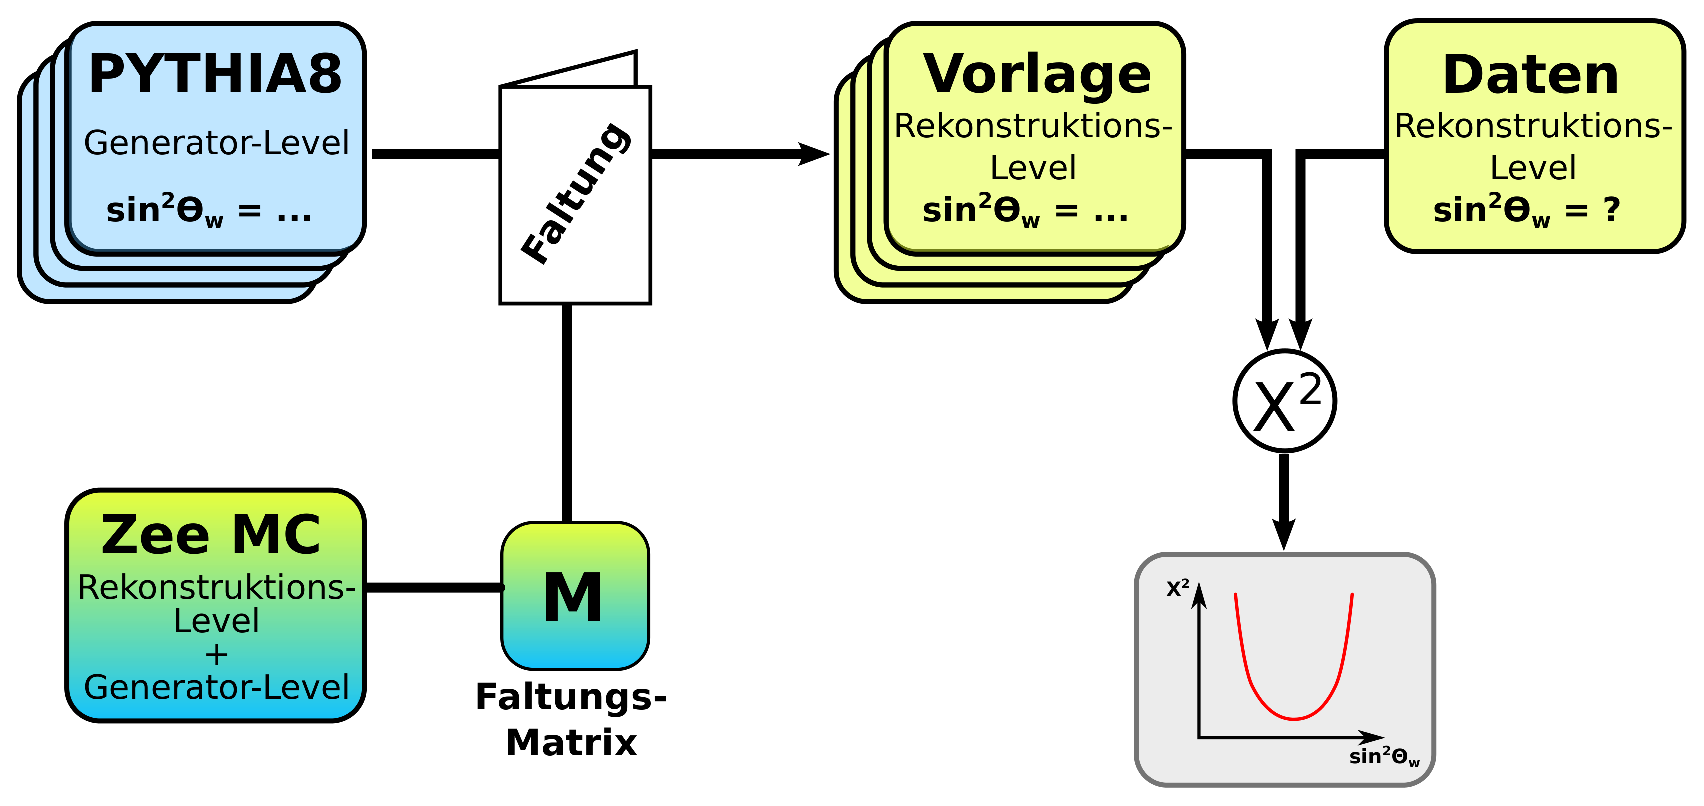
\includegraphics[width=1.0\textwidth]{img/templates}
    \caption[Schematische Darstellung des Extraktionsprozesses]
        {Schematische Darstellung des Extraktionsprozesses}
    \label{fig:templates}
\end{figure}

Die Simulation der Asymmetrie-Verteilungen für verschiedene Werte des schwachen
Mischungswinkels wird mit \textsc{Pythia8} durchgeführt\footnote{Wie schon in
obigen Abschnitt \ref{afb:dilution} wird hierfür die lokale Installation von
\textsc{Pythia8} verwendet, die keiner Verifikation durch die ATLAS Monte-Carlo
Workinggroup unterliegt} und erfolgt zunächst rein auf Generator-Level (blau in
Abb. \ref{fig:templates}). Mit \textsc{Pythia8} ist es möglich den Wert von
$\sin^2\theta_W$ und $\sin^2\theta_W^\text{eff,l}$ innerhalb fester Grenzen
($0,2250 \: ... \: 0,2400$) auf einen beliebigen Wert festzulegen. Für den
hiesigen Zweck wurden deshalb in Schritten von $0,0005$ beide Parameter
simultan variiert, wobei die in Gleichung (\ref{eq:effective_angle}) gezeigte
Differenz von $0,00029$ zwischen $\sin^2\theta_W$ und
$\sin^2\theta_W^\text{eff,l}$ stets beibehalten wurde. Für alle Einstellungen
wurden anschließend Datensätze mit je 10 Millionen Ereignissen im \ac{CC}-Kanal
und je 1 Million im \ac{CF}-Kanal simuliert. Dabei wurden für beide Kanäle
getrennte Konfigurationen für die Simulationen verwendet, um den
unterschiedlichen Phasenräumen beider Selektionen Rechnung zu tragen. Die
verwendete Konfiguration von \textsc{Pythia8} ist in Anhang
\ref{pythia8:templates} augeführt.

Um Vergleiche mit gemessenen Daten sinnvoll anstellen zu können bedarf es
aber noch der Berücksichtigung von Detektoreffekten, wie Auflösung, Akzeptanz
und Rekonstruktionseffizienz. Diese Aufgabe übernimmt normalerweise das in
Kapitel \ref{event_generation} erwähnte Paket \textsc{GEANT4} zur Simulation
der Detektorantwort, was jedoch äußert komplex und rechenintensiv ist. Aus
diesem Grund wird in dieser Arbeit ein anderer Ansatz gewählt. Man nutzt die
Tatsache aus, dass bei der Produktion des Signal Monte-Carlos neben den
rekonstruierten Größen (gelb in Abb. \ref{fig:templates}) auch die
darunterliegenden Generator-Level Informationen bekannt sind, sodass auf
statistischer Basis der Einfluss des Detektors einbezogen werden kann. Es wird
eine Matrix erzeugt, die den Übergang von Werten auf Generator-Level zu Werten
auf Rekonstruktions-Level repräsentiert.
\begin{equation}
    \bf r = M \cdot \bf{g}
    \label{eq:folding}
\end{equation}
Im Falle einer einzigen Observablen, beispielsweise der invarianten Masse des
Elektronpaares, wären $\bf{r}$ und $\bf{g}$ Histogramme der Massenspektren auf
Rekonstruktions- bzw. Generator-Level, mit jeweils $n$ Unterteilungen -
mathematisch dargestellt durch $n$-dimensionale Vektoren. Die Faltungsmatrix
$\bf{M}$ wäre somit von der Dimension $n \times n$. Für die Messung der
Vorwärts-Rückwärts Asymmetrie ist allerdings neben der invarianten Masse noch
der Emissionswinkel des Elektrons $\cos\theta_{cs}$ nötig, sodass die Objekte
in Gleichung (\ref{eq:folding}) erweitert werden müssen. Für $m$ Unterteilungen
der Histogramme von $\cos\theta_{cs}$ müssen $\bf{r}$ und $\bf{g}$ nun durch 
$n \times m$-Matrizen dargestellt werden, während $\bf{M}$ zu einem Tensor
vierter Stufe wird\footnote{der Einfachheit halber wird im Folgenden dennoch
der Begriff Faltungs\textit{matrix} für $\bf{M}$ verwendet}.

Tatsächlich wird die invariante Masse nach Tabelle \ref{tab:binning_afb} in 11
Bereiche unterteilt, während der Emissionswinkel lediglich nach
\textit{vorwärts} und \textit{rückwärts} ($=2$ Unterteilungen) unterschieden
wird. Zur Erstellung und Verwaltung von $\bf{M}$ wird das Software-Paket
\textsc{RooUnfold} (\cite{2011arXiv1105.1160A}) in der Version 1.1.1 verwendet.
Dieses bietet die Möglichkeit der komfortablen Erstellung einer solchen Matrix
und implementiert zudem Algorithmen zum Entfalten oder Falten statistischer
Verteilungen.

Die Faltung der oben beschriebenen Sätze von Generator-Level Verteilungen mit
variierten schwachen Mischungswinkeln mit der Faltungsmatrix $\bf{M}$ führt nun
also zu Verteilungs-Vorlagen, die zum Verglich mit real gemessen Daten
verwendet werden können. Abbildung \ref{fig:vorlage} zeigt beispielhaft die
Asymmetrie Verteilung einer solchen Vorlage.

\begin{figure}
    \centering
    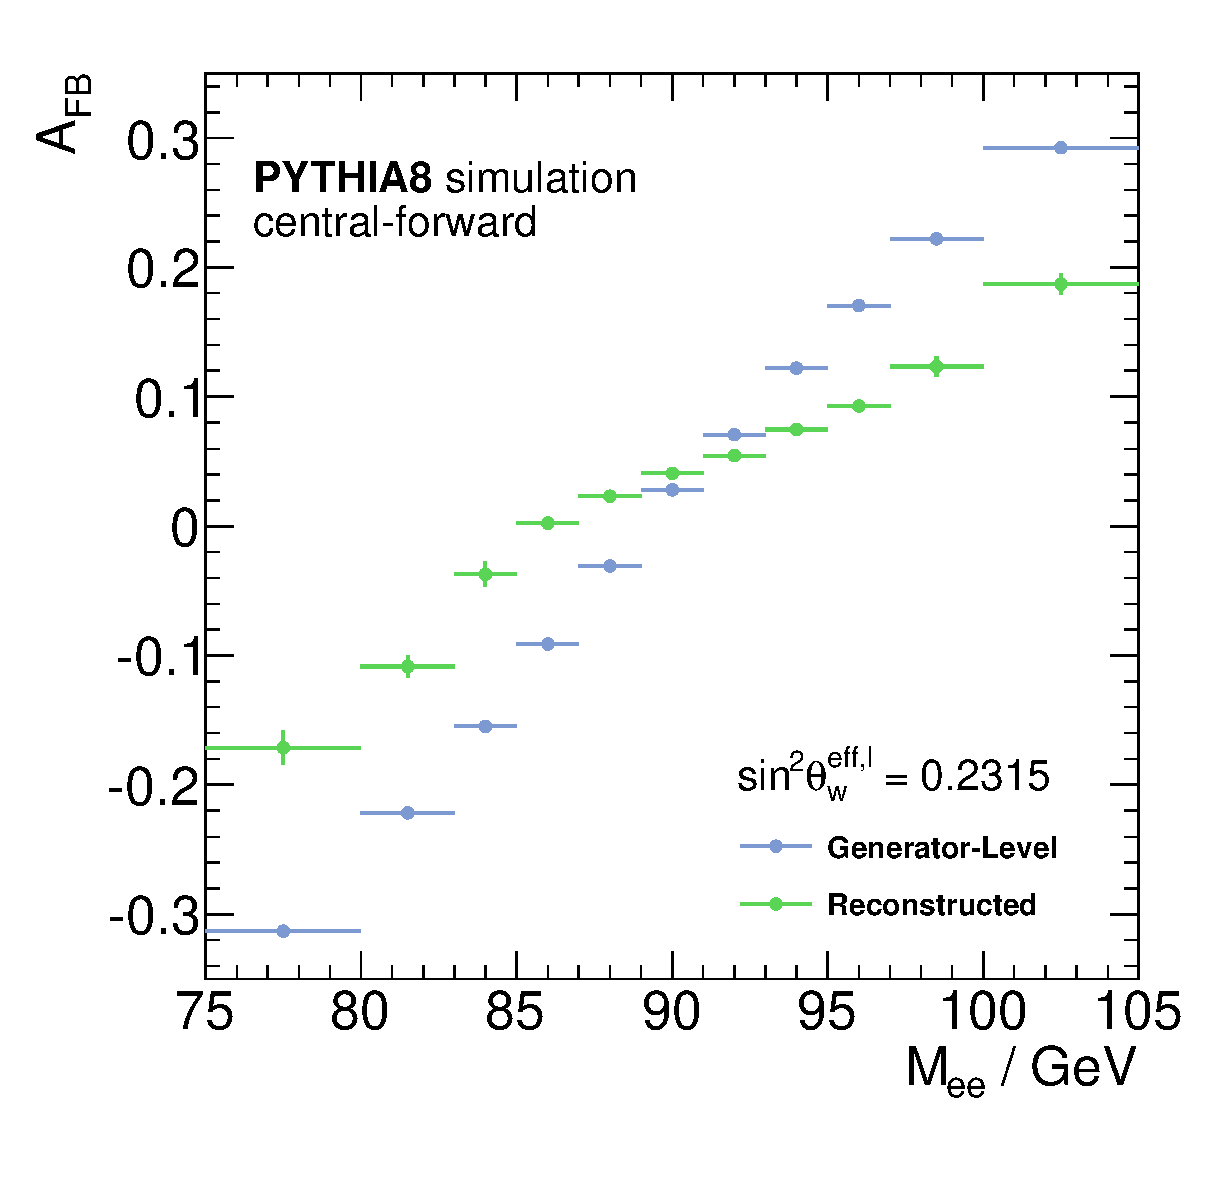
\includegraphics[width=0.48\textwidth]{plots/templates_cf_comp}
    \hfill
    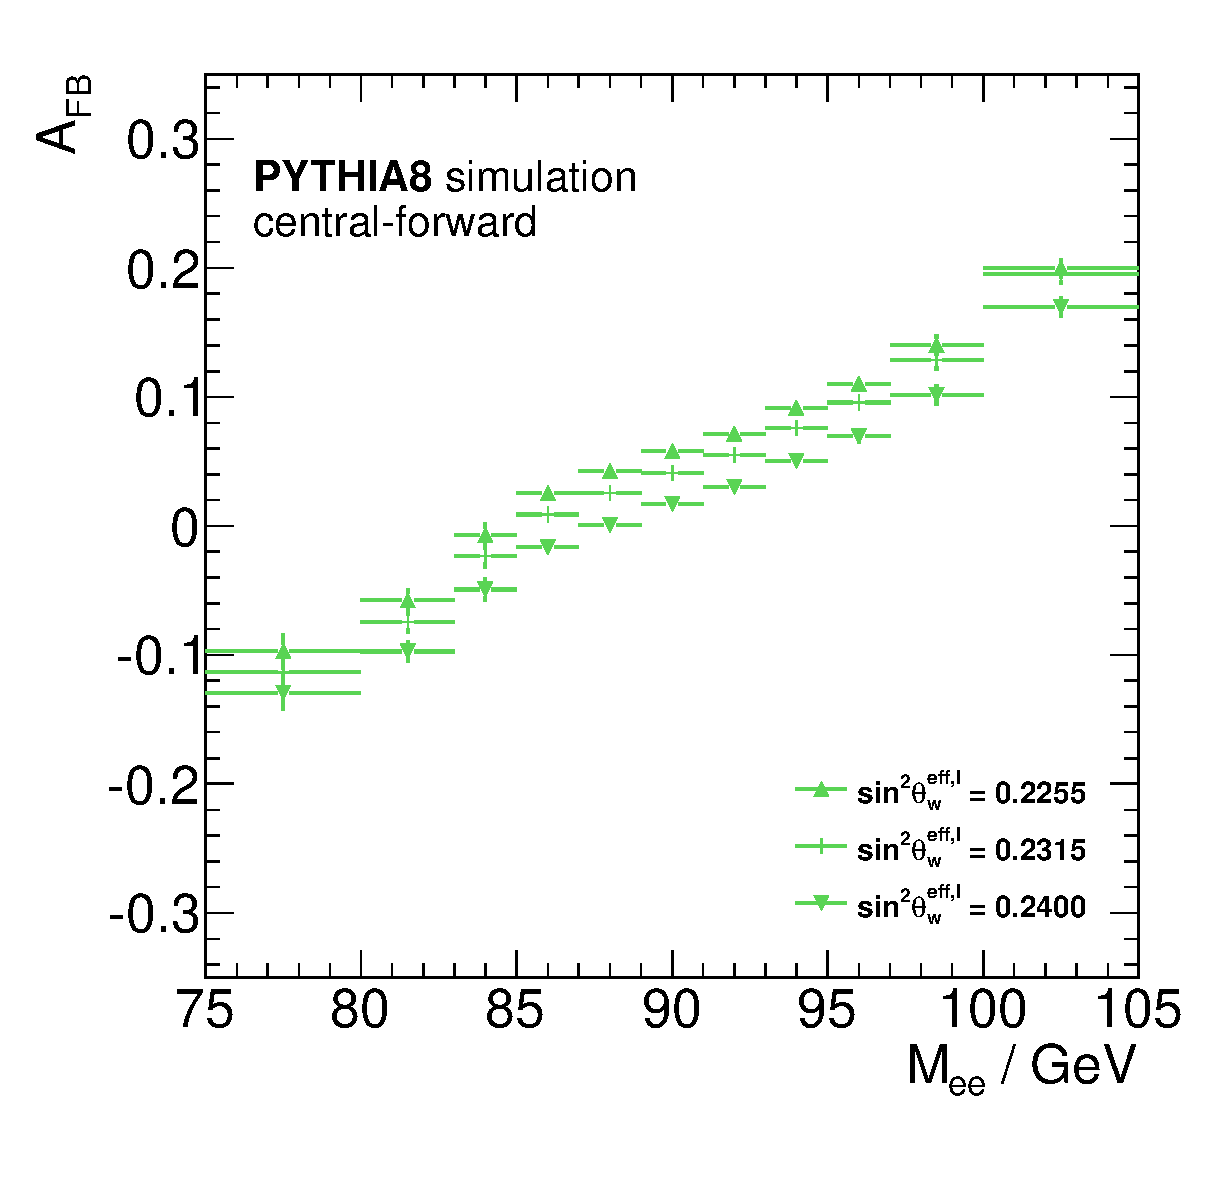
\includegraphics[width=0.48\textwidth]{plots/templates_cf}
    \caption[Asymmetrie-Vorlagen zur Extraktion des schwachen Mischungswinkels]
        {Asymmetrie-Vorlagen zur Extraktion des schwachen Mischungswinkels im
        \ac{CF}-Kanal. \textbf{Links:} Vergleich zwischen der
        Asymmetrie-Verteilung auf Generator-Level und nach Anwendung der
        Faltungsmatrix. \textbf{Rechts:} Asymmetire-Vorlagen nach Faltung für
        drei verschiedene Werte von $\sin^2\theta_W^\text{eff,l}$.}
    \label{fig:vorlage}
\end{figure}

Auf der linken Seite von Abb. \ref{fig:vorlage} ist der Vergleich zwischen der
Asymmetrie-Verteilung auf Generator-Level und nach der Asymmetrie nach
Anwendung der Faltungsmatrix, also mit Berücksichtigung von Detektoreffekten,
dargestellt. Man erkennt die deutliche Abschwächung der Asymmetrie
hervorgerufen von Migrationseffekten und Detektorineffizienzen (siehe voriger
Abschnitt \ref{afb:afb}). Zudem ist die am Ende des vorigen Abschnitts
beschriebe Änderung der Steigung um die Z-Masse nach der Einführung der
Detektoreffekte sehr deutlich zu beobachten. Auf der rechten Seite von Abb.
\ref{fig:vorlage} sind für den niedrigsten, den höchsten und den nominellen
Wert des effektiven schwachen Mischungswinkels die resultierenden
Asymmetrie-Vorlagen gezeigt. Letztere liegt dabei erwartungsgemäß zwischen den
beiden Vorlagen der Randwerte von $\sin^2\theta_W^\text{eff,l}$.

Die gezeigten Unsicherheiten sind rein statistischer Natur und beinhalten die
statistische Unsicherheit der Generator-Level Verteilungen, sowie die der
Faltungsmatrix. Um den Einfluss der
letztgenannanten Quelle abzuschätzen bedarf es einer besonderen Methode. Es
wird hierfür sogenanntes \textit{Bootstrapping} (\cite{zbMATH03631774})
benutzt, wobei jedem Ereignis, dass zum Füllen der Faltungsmatrix verwendet
wird ein individuelles, zufälliges Gewicht zugewiesen wird. Die Gewichte
folgen dabei insgesammt einer Poisson-Verteilung um 1, sodass die eingführte
Umgewichtung unitär ist und die Normierung der Matrix erhalten bleibt. Man
erstellt nun $n$ Faltungsmatrizen aus ein und dem selben Singal Monte-Carlo,
aber mit jeweils unterschiedlichen Sätzen an Ereignisgewichten.
Diese werden nun einzeln, wie oben beschrieben, zur Faltung der Generator-Level
Verteilungen verwendet, wodurch für jede dieser Verteilungen $n$
Asymmetrie-Vorlagen entstehen. Schlussendlich wird für jeden Massenbereich der
Mittelwert und die Standardabweichung aus den $n$ Vorlagen berechnet, um zur
finalen Asymmetrie-Vorlage zu gelangen.

Jede Vorlage eines Kanals\footnote{gemeint sind \ac{CC}- und \ac{CF}-Kanal}
muss nun mit der entsprechenden untergrundreduzierten Asymmetrie-Verteilung aus
Daten verglichen werden und die $\chi^2$ Teststatistik berechnet werden. Diese
ist definiert als
\begin{equation}
    \chi^2 \;=\; \sum_{i=1}^{N}
        \frac{
            \left(
                {(\afb^\text{data})}_i - {(\afb^\text{templ})}_i
            \right)^2
        }{
            (\sigma_i^\text{data})^2 + (\sigma_i^\text{templ})^2
        }
\end{equation}
wobei der Index $i$ über alle Bereiche $N$ der invarianten Masse läuft. Die
hochgestellten Indizes \textit{data} und \textit{templ} beziehen sich auf die
Asymmetrie-Verteilung ($\afb$) und die jeweilige Unsicherheit ($\sigma$) in
Daten bzw. den Vorlagen.



\subsection{Extraktion}
\label{afb:extraction}

% + Extraktion
%   - Template Fits
%   - Closure-Test
%   - Resultate (einzeln und kombiniert)

Vor der eigentlichen Messung des schwachen Mischungswinkels nach gerade
beschriebenem Prinzip, soll zuvor noch die Methode an sich verifiziert werden.
Dazu wird statt der Asymmetrie-Verteilung aus Daten die entsprechende
Verteilung des Signal Monte-Carlos verwendet und überprüft, ob die Prozedur den
Wert des schwachen Mischungswinkel reproduziert, mit dem die Simulation erzeugt
wurde. Abbildung \ref{fig:closure} zeigt die resultierenden
$\chi^2$-Verteilungen.

\begin{figure}[h]
    \centering
    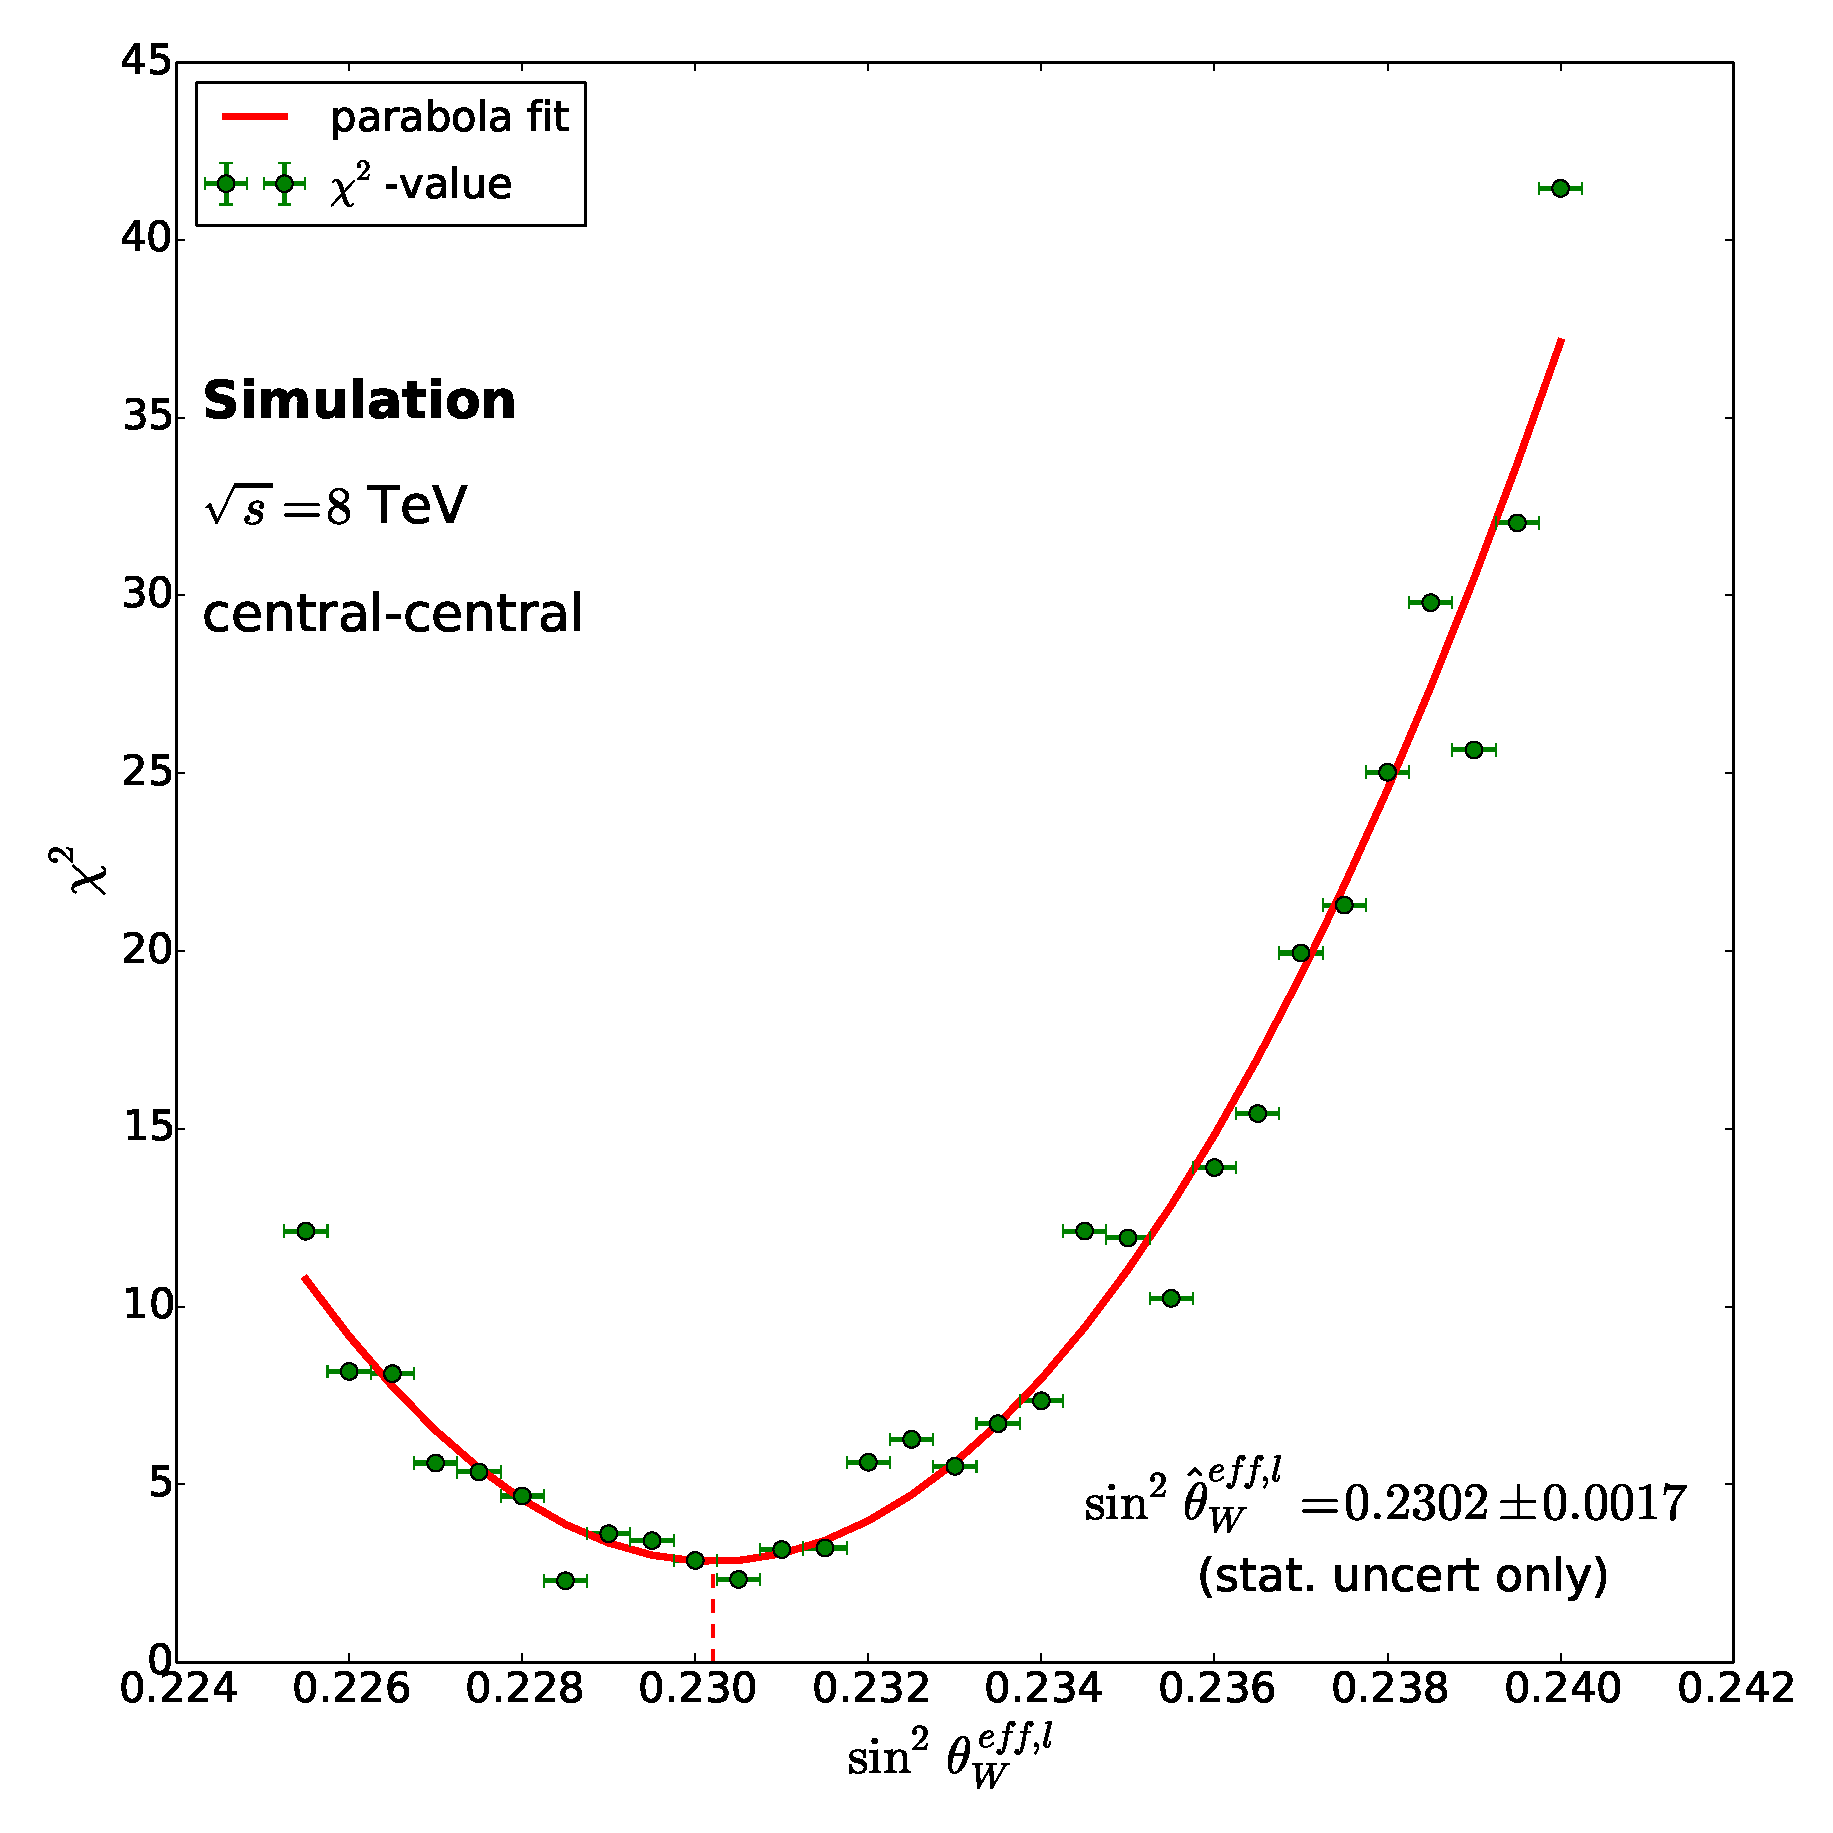
\includegraphics[width=0.48\textwidth]{plots/sin2theta_cc_closure}
    \hfill
    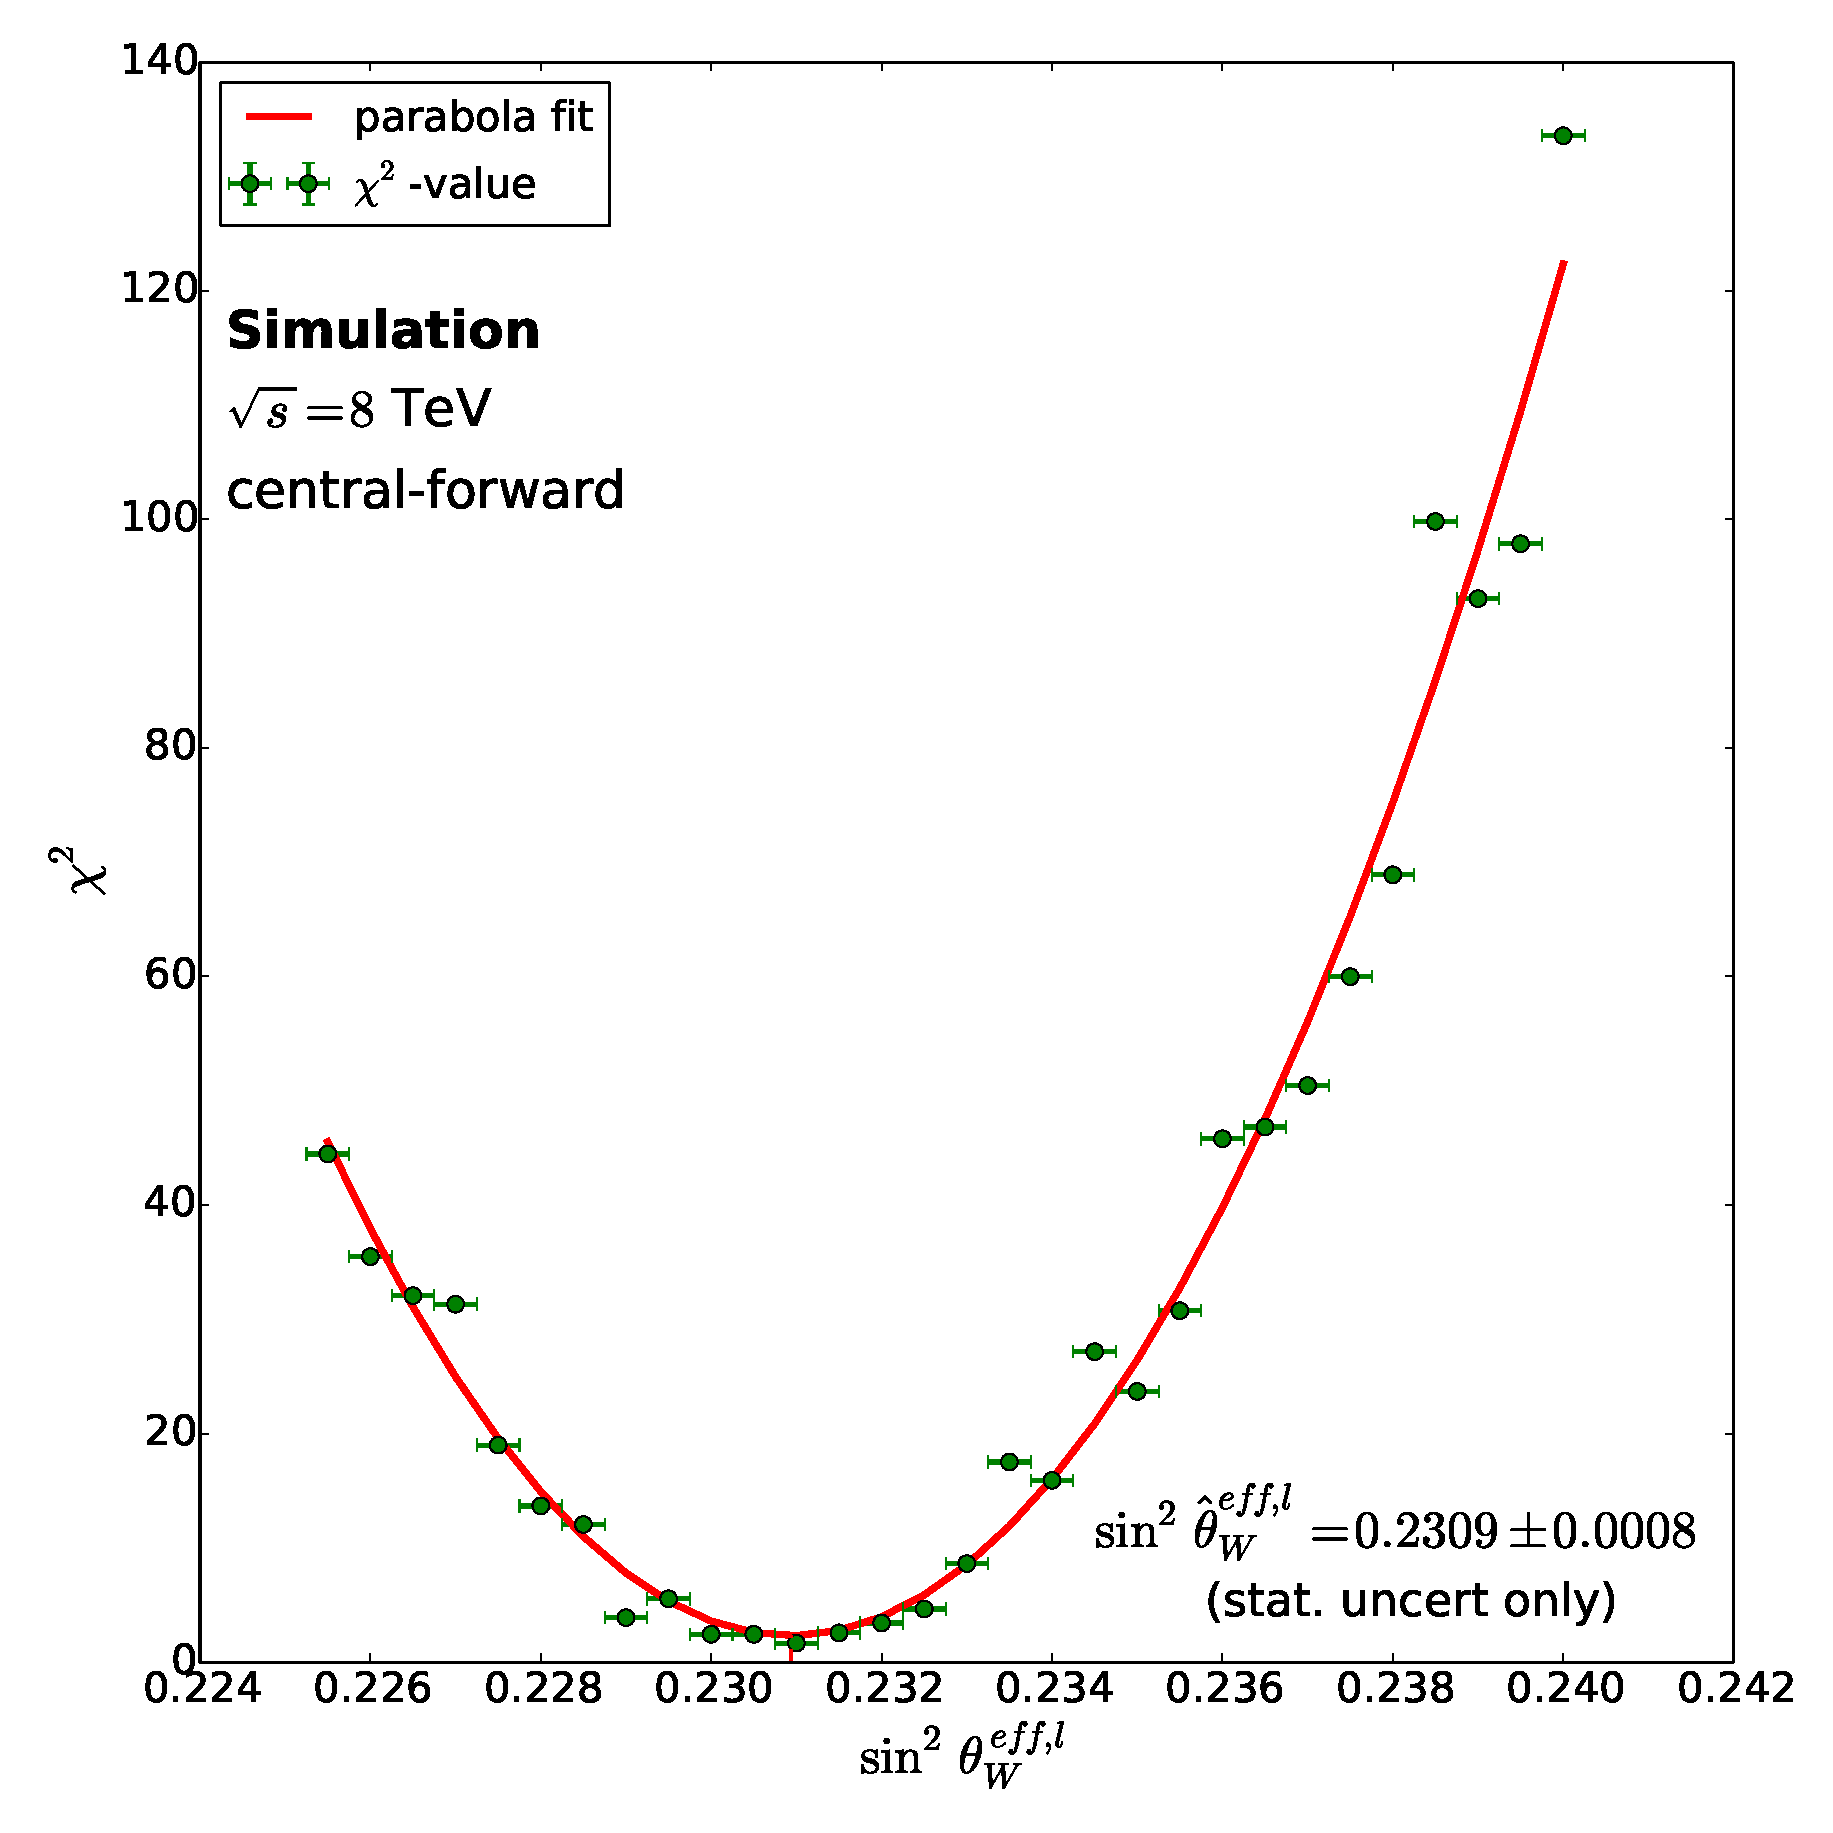
\includegraphics[width=0.48\textwidth]{plots/sin2theta_cf_closure}
    \caption[Extraktion des simulierten schwachen Mischungswinkels zur
        Verifikation der Methode]
        {Extraktion des simulierten schwachen Mischungswinkels zur
        Verifikation der Methode im \ac{CC}-Kanal (links) und \ac{CF}-Kanal
        (links)}
    \label{fig:closure}
\end{figure}

Die Kurvenanpassung der Parabel wurde mithilfe des quelloffenen Python Paketes
\textsc{SciPy} (\cite{scipy}) durchgeführt, wobei für die Parabel folgende
analytische Form gewählt wurde:
\begin{equation}
    f(x)=a+b\cdot(x-c)^2
    \label{eq:parabola}
\end{equation}
Der Parameter $c$ entspricht in dieser Parametrisierung dem Minimum der
Parabel, also dem Messwert für den schwachen Mischungswinkel. Die Unsicherheit
auf diesen Wert ergibt sich aus der Öffnung der Parabel, genauer dem Betrag der
Differenz zwischen der Stelle des Minimums und einem der Punkte, an denen die
Parabel auf $f(x_\text{min})+1$ angestiegen ist:
\begin{align}
    \sigma \;&=\; |x_\text{min} - x_{1,2}|
        \qquad \text{mit:} \quad f(x_{1,2}) = f(x_\text{min})+1
        \\[5pt]
    \Longrightarrow \quad \sigma \;&=\; \sqrt{\frac{1}{b}}
    \label{eq:sigma}
\end{align}
Gleichung (\ref{eq:sigma}) zeigt bereits den analytischen Ausdruck, dieser
Unsicherheit, der sich aus der Form (\ref{eq:parabola}) ableiten lässt.

Die beiden aus der Extraktion resultierenden Werte für den schwachen
Mischungswinkel sind in Abb. \ref{fig:closure} jeweils rechts unten gezeigt.
Bei deren Betrachtung fällt zunächst auf, dass die Unsicherheit im
\ac{CC}-Kanal größer ist, als im \ac{CF}-Kanal, was an der im Zentral-Bereich
viel stärker ausgeprägten Abschwächung der Asymmetrie durch
Dilution-Effekte\footnote{siehe Abschnitt \ref{afb:dilution} und Abbildung
\ref{fig:dilution}} begründet liegt. Für die sonstige Fluktuation der Punkte um
die Parabel, existieren mehrere mögliche Quellen. Zum einen könnte die
limitierte Statistik des Signal Monte-Carlos, welches hier zur Verifikation und
zur Erstellung der Faltungsmatrix verwendet wird. Das gleiche Argument gilt
aber auch für die Vorlagen an sich und würde sich somit auch für die
eigentliche Extraktion aus Daten Bestand haben. Berechnet man das reduzierte
$\chi^2_\text{red}$ aus dem Wert am Minimum ($\chi^2_\text{min} = a$), geteilt
durch die Anazahl der Freiheitsgrade ($n_\text{dof} = 11$, siehe Tabelle
\ref{tab:binning_afb}) so ergibt sich im \ac{CC}-Kanal eine Wert von $0,26$
und im \ac{CF}-Kanal von $0,21$, was insgesammt für eine gute Qualität der
Anpassung spricht. Der nominelle Wert des schwachen Mischungswinkels, mit dem
das Signal Monte-Carlo erstellt wurde, entspricht dem Welt-Mittelwert von
$\sin^2\theta_W^\text{eff,l}=0,23146$. Die extrahierten Werte nach obiger
Prozedur stimmen somit im Rahmen der angegebenen Toleranzen mit diesem Wert
überein, was die Anwendung der Methode zur Extraktion aus realen Daten
legitimiert. Dennoch bleiben die beobachteten großen Unsicherheiten und die
Fluktuationen innerhalb der $\chi^2$-Verteilungen kritisch zu
hinterfragen\footnote{Eine Diskussion der vorgestellten Methode und potentielle
Verbesserungsmöglichkeiten schließt sich nach der Präsentation der Ergebnisse
aus den Daten, am Ende dieses Kapitel an}.

Nach der Verifikation der Extraktionsprozedur wird diese nun auf die
Asymmetrie-Vertei"-lungen der Daten angewendet. Abbildung \ref{fig:sin2theta}
zeigt die entstehende $\chi^2$-Verteilungen beider Kanäle.
\begin{figure}[p]
    \centering
    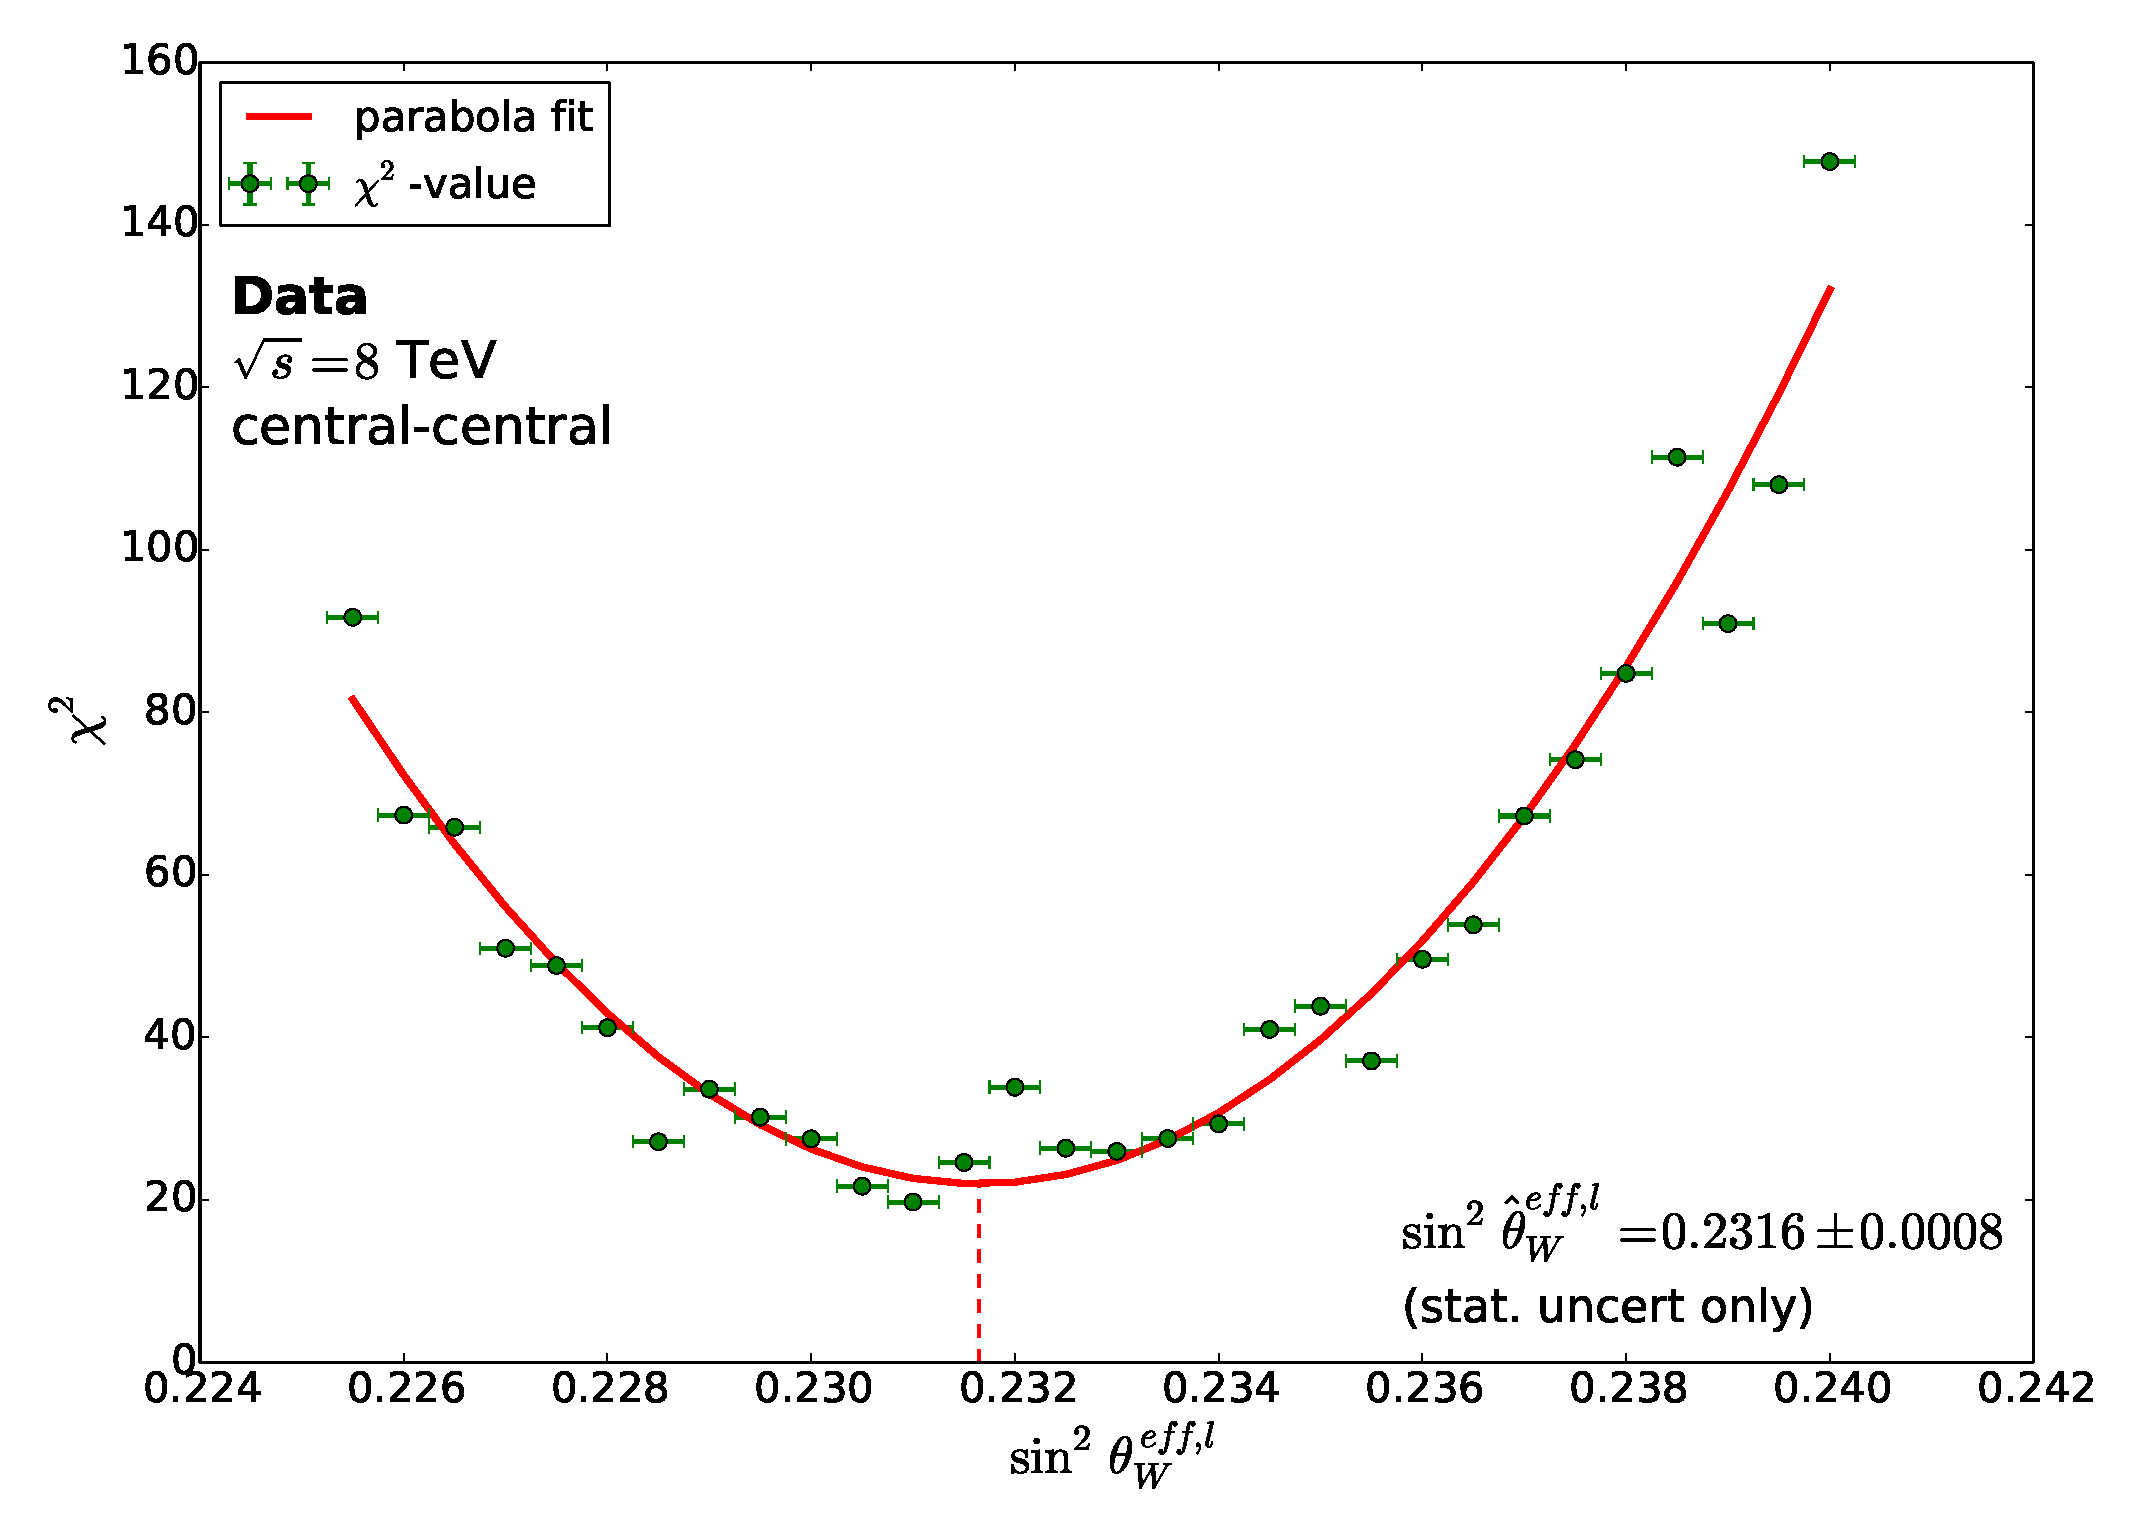
\includegraphics[width=1.0\textwidth]{plots/sin2theta_cc_data}

    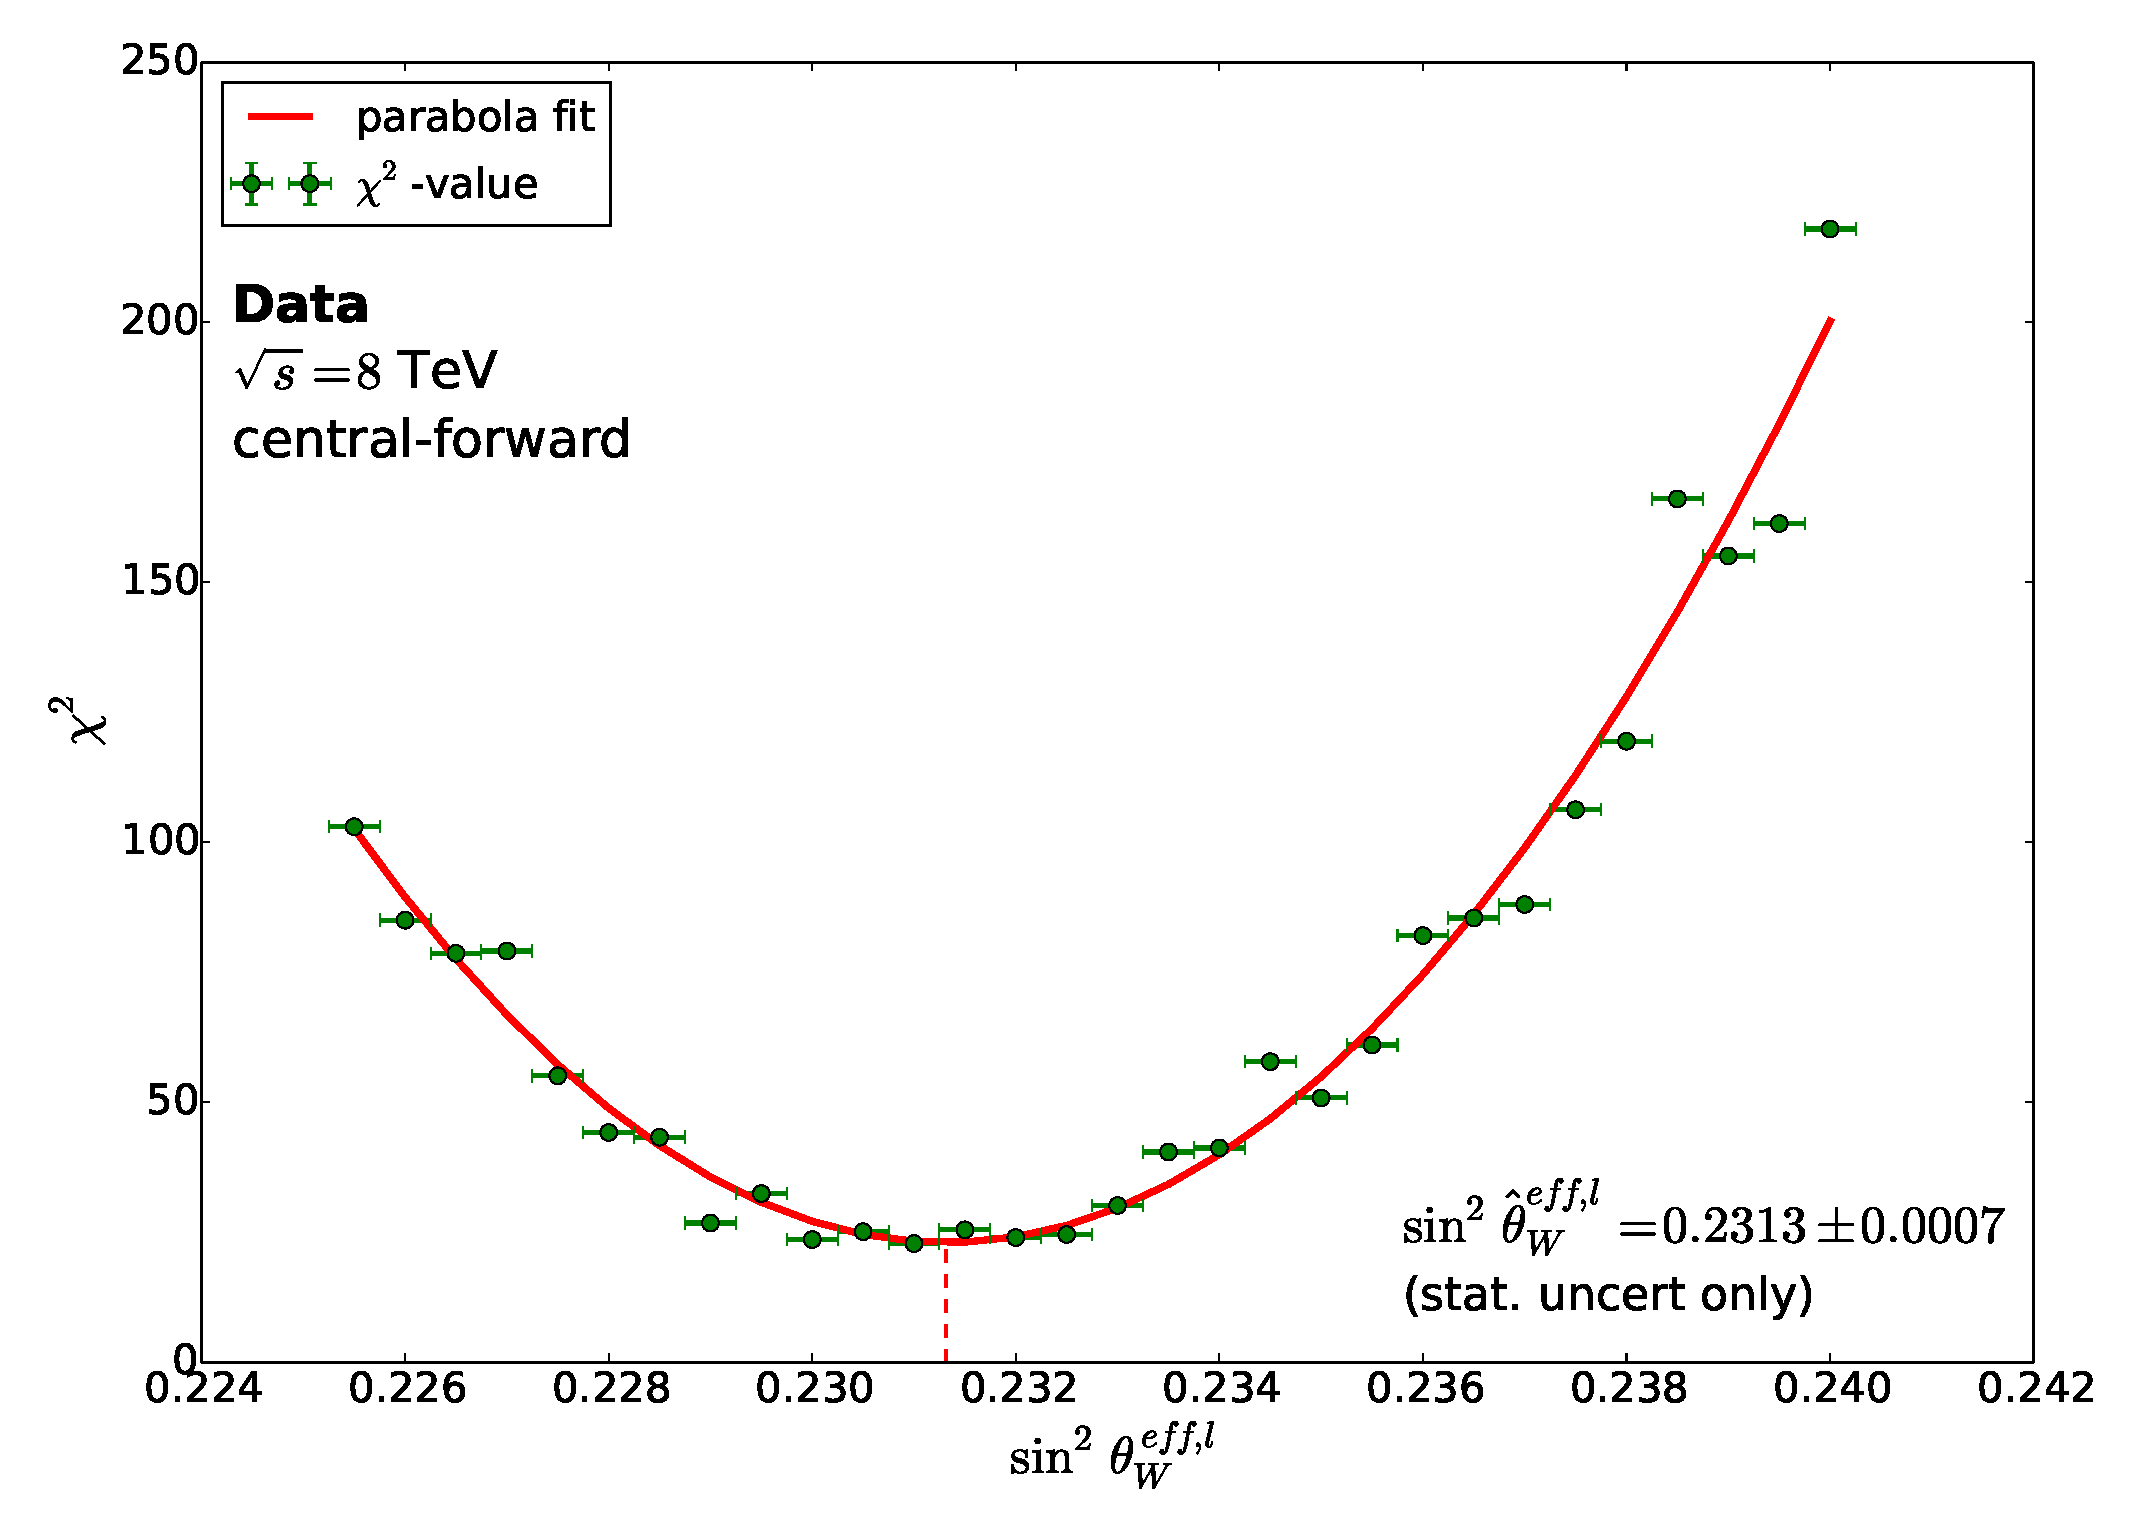
\includegraphics[width=1.0\textwidth]{plots/sin2theta_cf_data}
    \caption[Extraktion des schwachen Mischungswinkels aus Verteilungen der
        Asymmetrie in Daten]
        {Extraktion des schwachen Mischungswinkels aus Verteilungen der
        Asymmetrie in Daten im \ac{CC}-Kanal (links) und \ac{CF}-Kanal
        (rechts)}
    \label{fig:sin2theta}
\end{figure}
Die aus der Anapassung der Parabel an die $\chi^2$-Verteilungen gewonnenen
Werte für den schwachen Mischungswinkel ergeben sich zu:
\begin{align*}
    \sin^2\theta_W^\text{eff,l (CC)} &\;=\; 0.2316
        \;\pm\; 0.0008 \;\text{(stat)}
    \\[5pt]
    \sin^2\theta_W^\text{eff,l (CF)} &\;=\; 0.2313
        \;\pm\; 0.0007 \;\text{(stat)}
\end{align*}
Auch hier zeigt sich das bereits erwartete Verhalten, dass die Unsicherheit auf
den Wert des schwachen Mischungswinkels im \ac{CC}-Kanal größer ist, als im
\ac{CF}-Kanal. Insgesammt jedoch haben sich die Unsicherheiten im Vergleich zur
vorangegangen Überprüfung mit dem Signal Monte-Carlo verkleinert, was an der
höheren statisitschen Signifikanz der Daten liegt. Die Werte für das reduzierte
$\chi^2_\text{red}$ ergeben sich hier zu $2,2$ für \ac{CC} und zu $2,1$ für
\ac{CF} und liegen somit im Rahmen einer zufreidenstellenden Beschreibung.
Wie schon beim Signal Monte-Carlo wird hier allerdings in ähnlichem Maße eine
gewisse Fluktuation der $\chi^2$-Werte um die Parabel beobachtet, was nun am
ehesten auf die statistische Signifikanz der der Vorlagen und der
Faltungsmatrix zurückzuführen ist.

Durch die Zusammenfassung der Ergebnisse beider Kanäle zu einem kombinierten
Messergebnis 
\begin{equation}
    \sin^2\theta_W^\text{eff,l} \;=\; 0.2314
        \;\pm\; 0.0005 \;\text{(stat)}
\end{equation}
kann die statistische Unsicherheit noch reduziert werden. Wie schon bei der
Messung der Vorwärts-Rückwärts Asymmetrie blieb im Rahmen dieser Arbeit kein
Raum zum Studium systematischer Einflüsse auf dieses Ergebnis. Eine qualitative
Diskussion erfolgt ebenso wie der Vergleich dieses Wertes mit vorangegangenen
Experimenten im folgenden Abschnitt.



\subsection{Diskussion und Ausbklick}
\label{afb:diskussion}

In diesem Kapitel wurde die Vermessung der Vorwärts-Rückwärts Asymmetrie im
Drell-Yan Prozess am $Z$-Pol und die anschließende Extraktion des effektiven
schwachen Mischungswinkels mittels Vorlagen-Tests präsentiert.

Der resultierende Wert von $\sin^2\theta_W^\text{eff,l}=0.2314\pm0.0005
\text{(stat)}$ soll nun in den Kontext früherer Messungen gesetzt werden. Die
bis heute genauesten Messungen des schwachen Mischungswinkels konnten in
Elektron-Positron Kollisionen durch LEP\footnote{\acf{LEP}} und
SLD\footnote{\acf{SLD}} erzielt werden, die ebenfalls die Vorwärts-Rückwärts
Asymmetrie am $Z$-Pol in leptonischen und hadronischen Endzuständen
untersuchten. Bei \ac{SLD} wurde darüber hinaus in Kollsisionen polarisierter
Elektronen mit unpolarisierten Positronen die Links-Rechts Asymmetrie zur
Bestimmung des schwachen Mischungswinkels verwendet. Zieht man alle Experimente
in betracht ergibt sich ein Mittelwert von $0,23069\pm0,00020$
(\cite{PhysRevD.86.010001}) für \ac{SLD} und $0,23181\pm0,00028$
(\cite{PhysRevD.86.010001}) für \ac{LEP}. In Hadron-Kollisionen konnte am
Tevatron\footnote{Proton-Antiproton Kollsisionen} mit dem D0-Detektor ein Wert
von $0,2309\pm0,0010$ (\cite{Abazov:2011ws}) für den schwachen Mischungswinkel
bestimmt werden. Dazu wurden in ähnlicher Weise Vorlagen-Tests verwendet, wie
es in der vorliegenden Arbeit der Fall ist. Ebenfalls am \ac{LHC} wurde mit den
2011 aufgenommenen Daten in Proton-Proton Kollisionen durch \acs{CMS} der
schwache Mischungwinkel auf $0,2287\pm0,0032$ (\cite{Chatrchyan:2011ya})
bestimmt. Zusammengefasst ergibt sich derzeit ein Weltmittelwert von
$0,23146\pm0,00012$ (\cite{PhysRevD.86.010001}), mit dem die vorliegende
Messung innerhalb der Unsicherheiten übereinstimmt. Abbildung
\ref{fig:results_comparison} fasst alle genannten Werte nochmals in einer
Übersicht zusammen.

\begin{figure}[h]
    \centering
    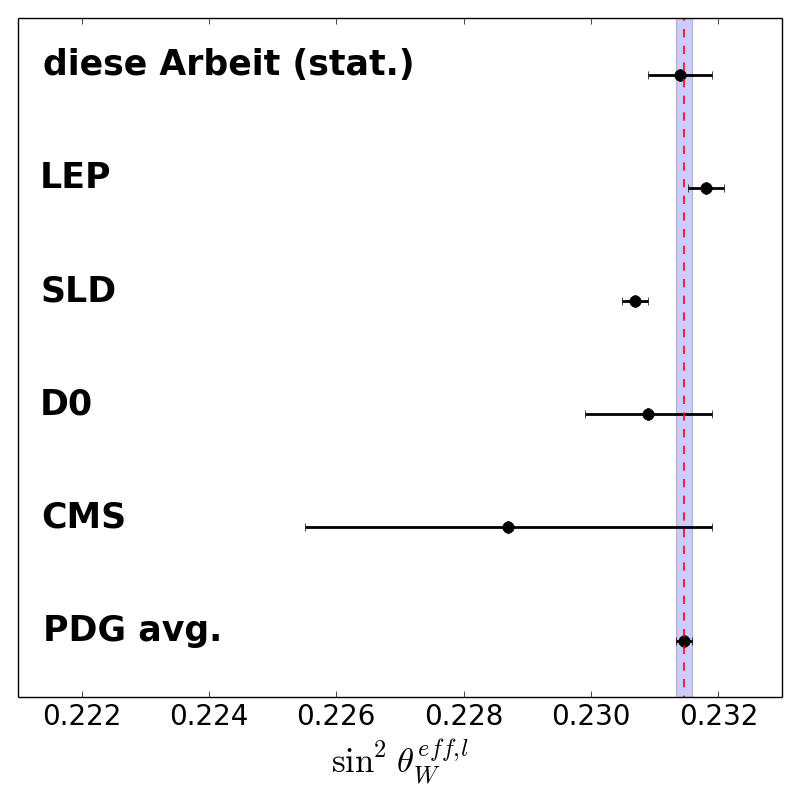
\includegraphics[width=0.6\textwidth]{plots/sin2theta_comparison}
    \caption[Werte des effektiven schwachen Mischungswinkels aus vorherigen
        Experimenten]
        {Werte des effektiven schwachen Mischungswinkels aus vorherigen
        Experimenten und der dieser Arbeit}
    \label{fig:results_comparison}
\end{figure}

Bei der Einordnung des resultierenden Wertes dieser Arbeit in den Kontext der
vorangegangenen Experimente bleibt allerdings zu beachten, dass keinerlei
systematischer Einflüsse auf diesen Wert Brücksichtigung gefunden haben. Wie
schon am Ende von Abschnitt \ref{afb:distributions} erläutert haben vor allem
die Wahl der \ac{PDF} und die Energiekalibration der Elektronen den größten
Einfluss auf die Verteilung der Vorwärts-Rückwärts Asymmetrie und somit auch
auf die Extraktion des schwachen Mischungswinkels. Der Einfluss der \ac{PDF}
schlägt sich bei der verwendeten Methode zusätzlich noch in der Erzeugung der
Vorlagen\footnote{siehe Anschnitt \ref{afb:extraction_method}} nieder, da sie
zum einen die Generator-Level Vorlagen selbst aber auch das zur Erstellung der
Faltungsmatrix verwendete Signal Monte-Carlo formen. Desweiteren spielt gerade
bei der Erstellung der Vorlagen die Anzahl der simulierten Ereignisse eine
tragende Rolle. Auf Seiten der Generator-Level Vorlagen als auch auf Seiten der
Faltungsmatrix bestimmt diese die statistische Signifikanz. Die in Abschnitt
\ref{afb:extraction} beobachteten Flukuationen der $\chi^2$-Punkte um die
Parabel wird durch diese bestimmt. Beim Vergleich der Asymmetrie-Verteilungen
der Vorlagen und Daten kommt bei letztgenannter auch die Qualität der
Abschätzung von Untergrundbeiträgen zum tragen. Insbesondere die datengestützte
Methode zur Ermittlung von Beiträgen der \ac{QCD} trifft stark vereinfachende
Annahmen und induziert somit zusätzliche Unsicherheiten systematischer Art.
Hier würde die Wahl einer suffizienteren Methode eine mögliche Verbesserung
darstellen.

Insgesammt konnte gezeigt werden, dass die vorgestellte Methode zur Extraktion
des schwachen Mischungswinkels zufriedenstellende und mit anderen Experimenten
vergleichbare Werte liefert.

